\documentclass[utf8x, notes, graphics]{beamer}
%\usepackage[norsk]{babel}
\usepackage[utf8x]{inputenc}
\usepackage[T1]{fontenc}
\usepackage[absolute,overlay]{textpos}
\usepackage{tikz}
\usepackage{chemfig}
\usepackage{xparse}
\usepackage{xifthen}
\usepackage{xcolor}
\usepackage{calc}
\usepackage{fp}
\usepackage{textpos}
\usepackage{graphicx}
\usepackage{eso-pic}
\usepackage{verbatim}

\usetikzlibrary{calc, arrows,shapes, intersections, decorations.pathreplacing, decorations.text, decorations.pathmorphing, decorations.fractals, patterns}
\tikzstyle{every picture}+=[remember picture]
\tikzstyle{na} = [baseline=-.5ex]
\usepackage{pgfplots}

\beamertemplatenavigationsymbolsempty

\definecolor{myGray}{rgb}{.5,.5,.5}
\setlength{\TPHorizModule}{\textwidth}
\setlength{\TPVertModule}{\textheight}
\newcommand{\myref}[1]{%
\begin{textblock}{1}[0,1](0.01,1.103)
\tiny{\color{myGray}{#1}}
\end{textblock}}

\newcommand{\zerodisplayskips}{%
  \abovedisplayskip=0pt
  \belowdisplayskip=0pt
  \abovedisplayshortskip=0pt
  \belowdisplayshortskip=0pt
}

\usefonttheme{professionalfonts}
\setbeamerfont{note page}{family*=pplx,size=\footnotesize} % 


\useoutertheme[subsection=false, footline=empty]{miniframes}
\useinnertheme{rectangles}
\usecolortheme{dolphin}
\usecolortheme{rose}
\setbeamercolor{frametitle}{bg=section in head/foot.bg!20!white}


\setbeamercovered{transparent}


\title{Molekylær modellering av oppsprekking i gasshydrater}
\author{Henrik Andersen Sveinsson}
\institute[Universitetet i Oslo] % (optional, but mostly needed)
{ Fysisk institutt\\
Det matematisk-naturvitenskapelige fakultet \\
Universitetet i Oslo
}
\date{8. mai 2015}

\AtBeginSection[]
{
  \begin{frame}<beamer>{Oversikt}
    \tableofcontents[currentsection]
  \end{frame}
}

\begin{document}
\begin{frame}
	\titlepage
\end{frame}

\begin{frame}
\frametitle{Oversikt}
\tableofcontents
\end{frame}

\section[Introduksjon]{Introduksjon og Bakgrunn}

\subsection{}

\begin{frame}
\frametitle{Hva gjør jeg i masteren min?}
Jeg kombinerer 3 ting som ikke er så vanlig å kombinere:
\begin{figure}
\begin{tikzpicture}[decoration={random steps,segment length=3pt,amplitude=2pt}]
\node (gashydrate) at (0, 0) {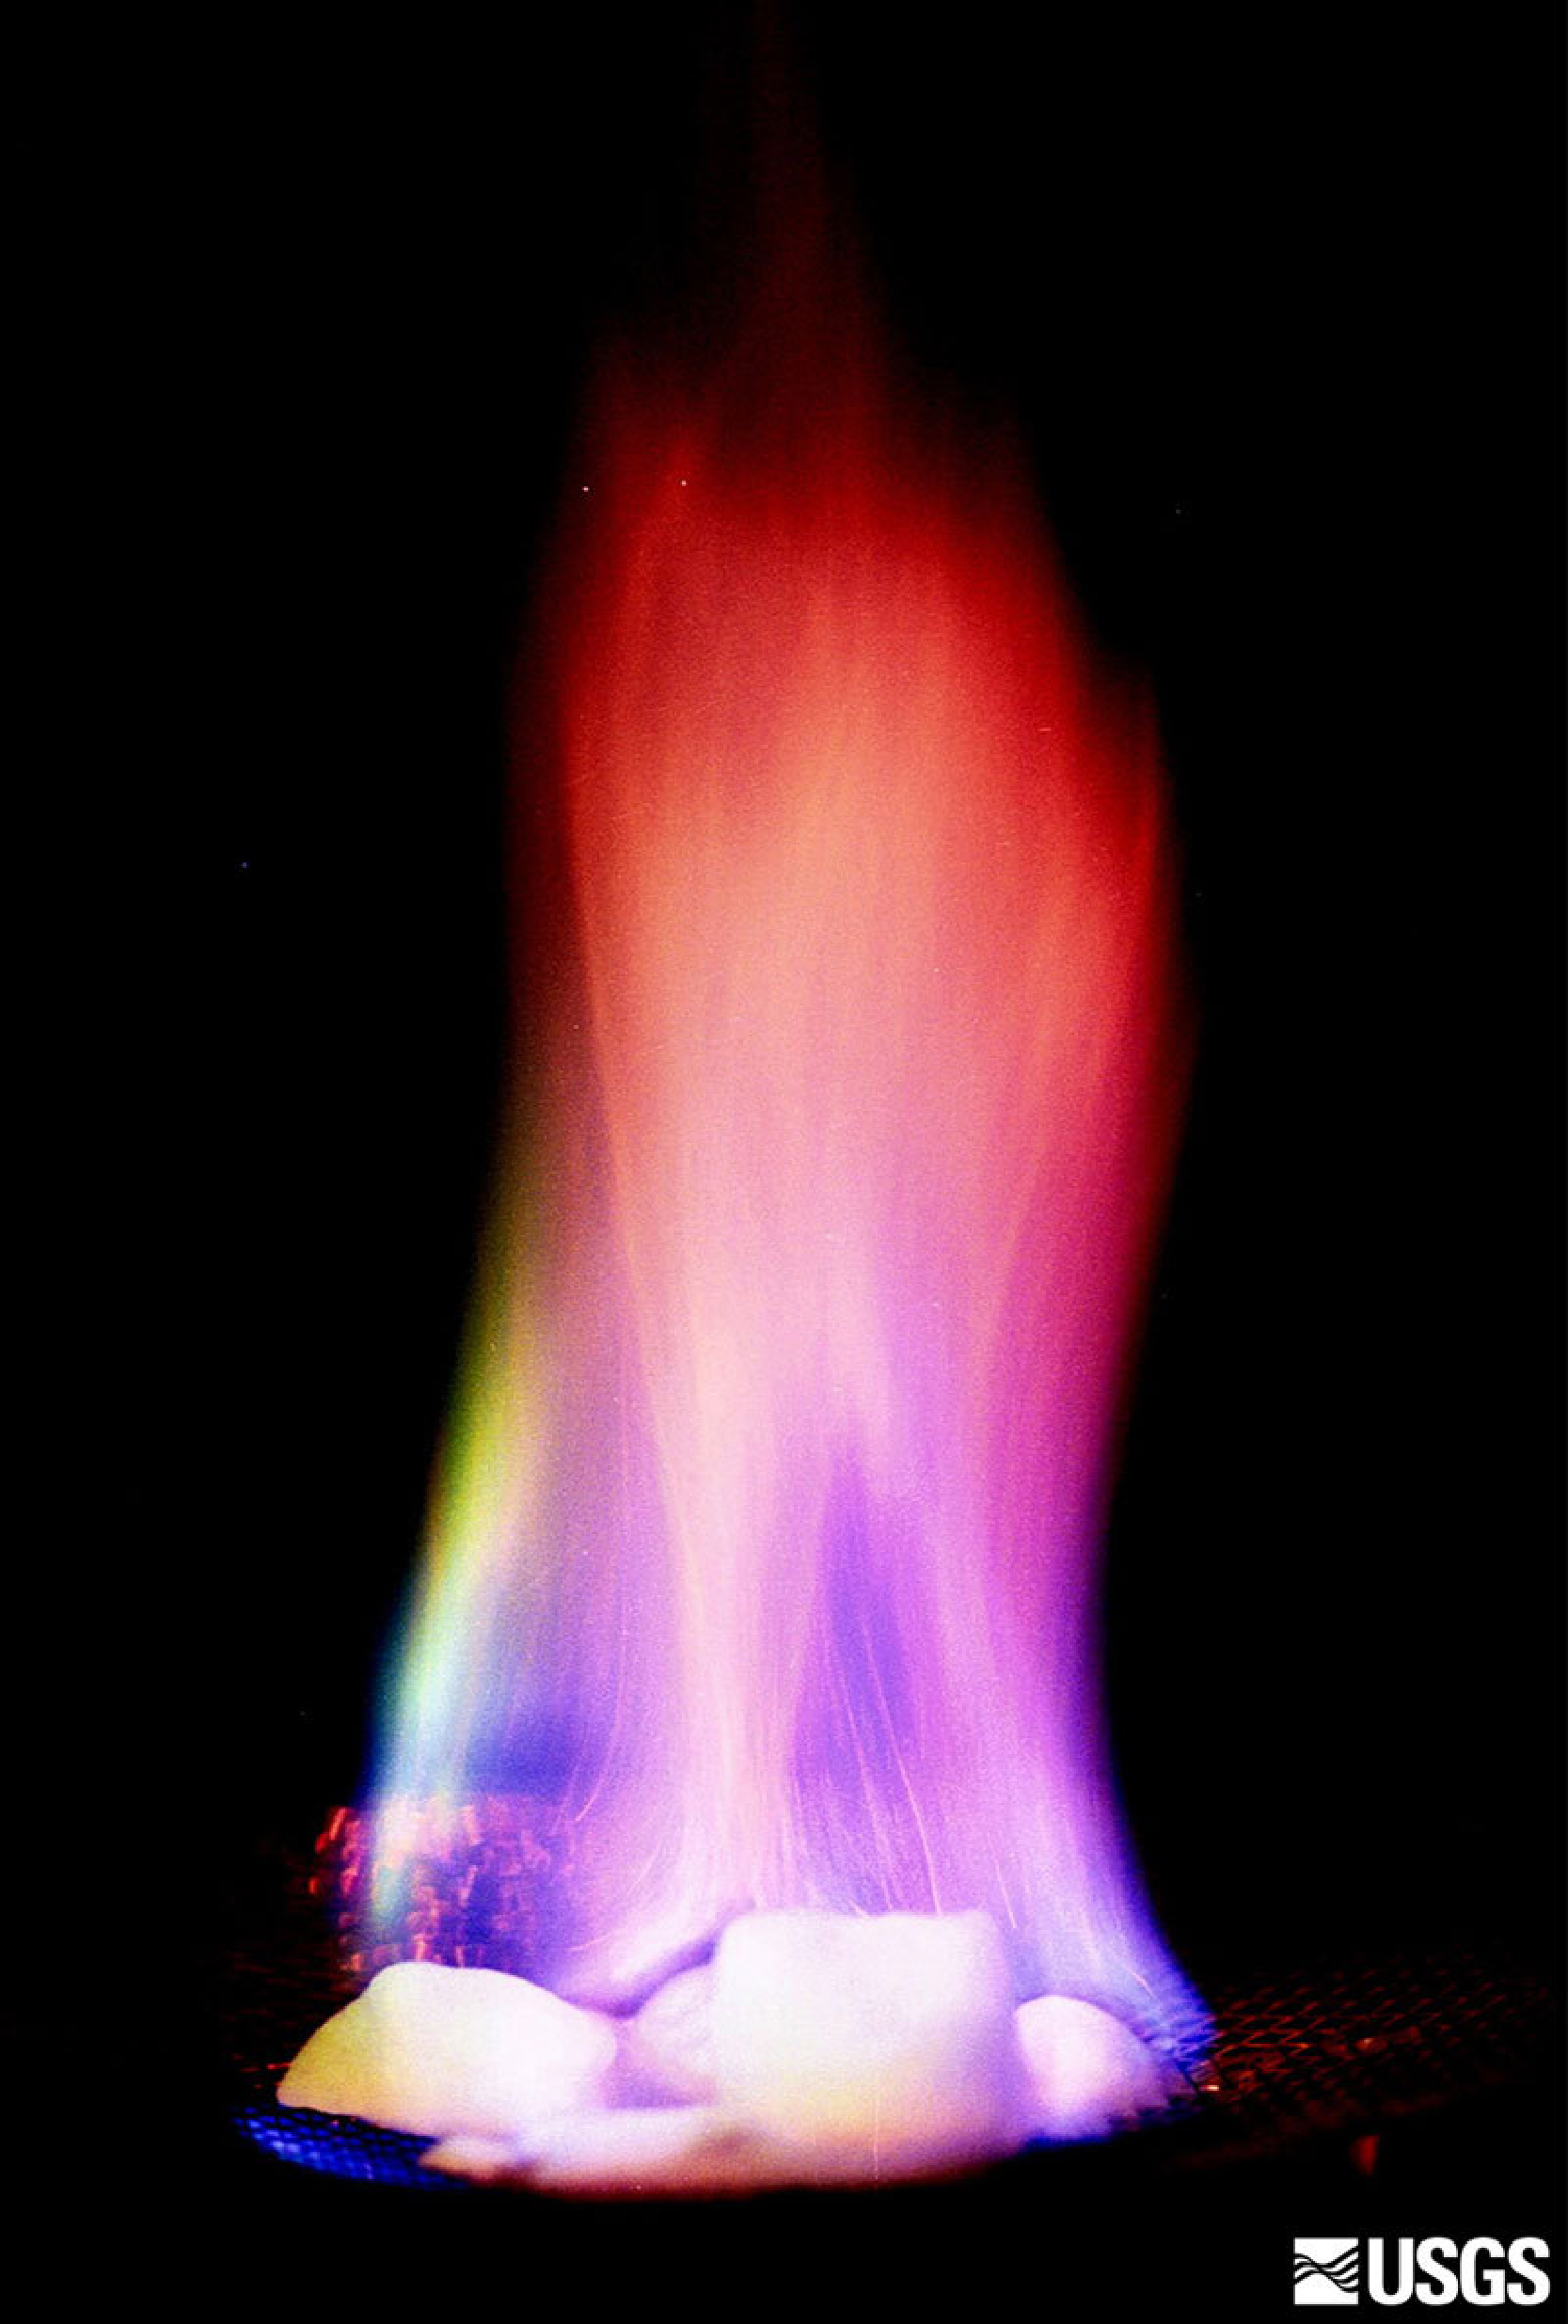
\includegraphics[width=0.2\textwidth]{../pictures/burning_hydrate.pdf}};
\begin{scope}[shift={(2, 1)}]
\draw[blue!40!white] (0, 0) rectangle (2, 3);
\pgfmathsetseed{1138}
\foreach \i in {1, 2, ..., 100}
{
\pgfmathrandominteger{\x}{0}{200}
\pgfmathrandominteger{\y}{0}{300}
\filldraw [red] (\x/100, \y/100) circle (1pt);
}
\end{scope}
\begin{scope}[shift={(5,-2)}]
\fill[color=blue!40!white] (0, 0) rectangle (2, 3);
\fill[white,decorate,rounded corners=1pt] (0,1.5) ellipse (1.5cm and 0.1cm);
\end{scope}
\end{tikzpicture}
\end{figure}
\end{frame}

\begin{frame}
\frametitle{Hva er gasshydrater?}
\begin{columns}[cc]
\column{0.5\textwidth}
\begin{figure}
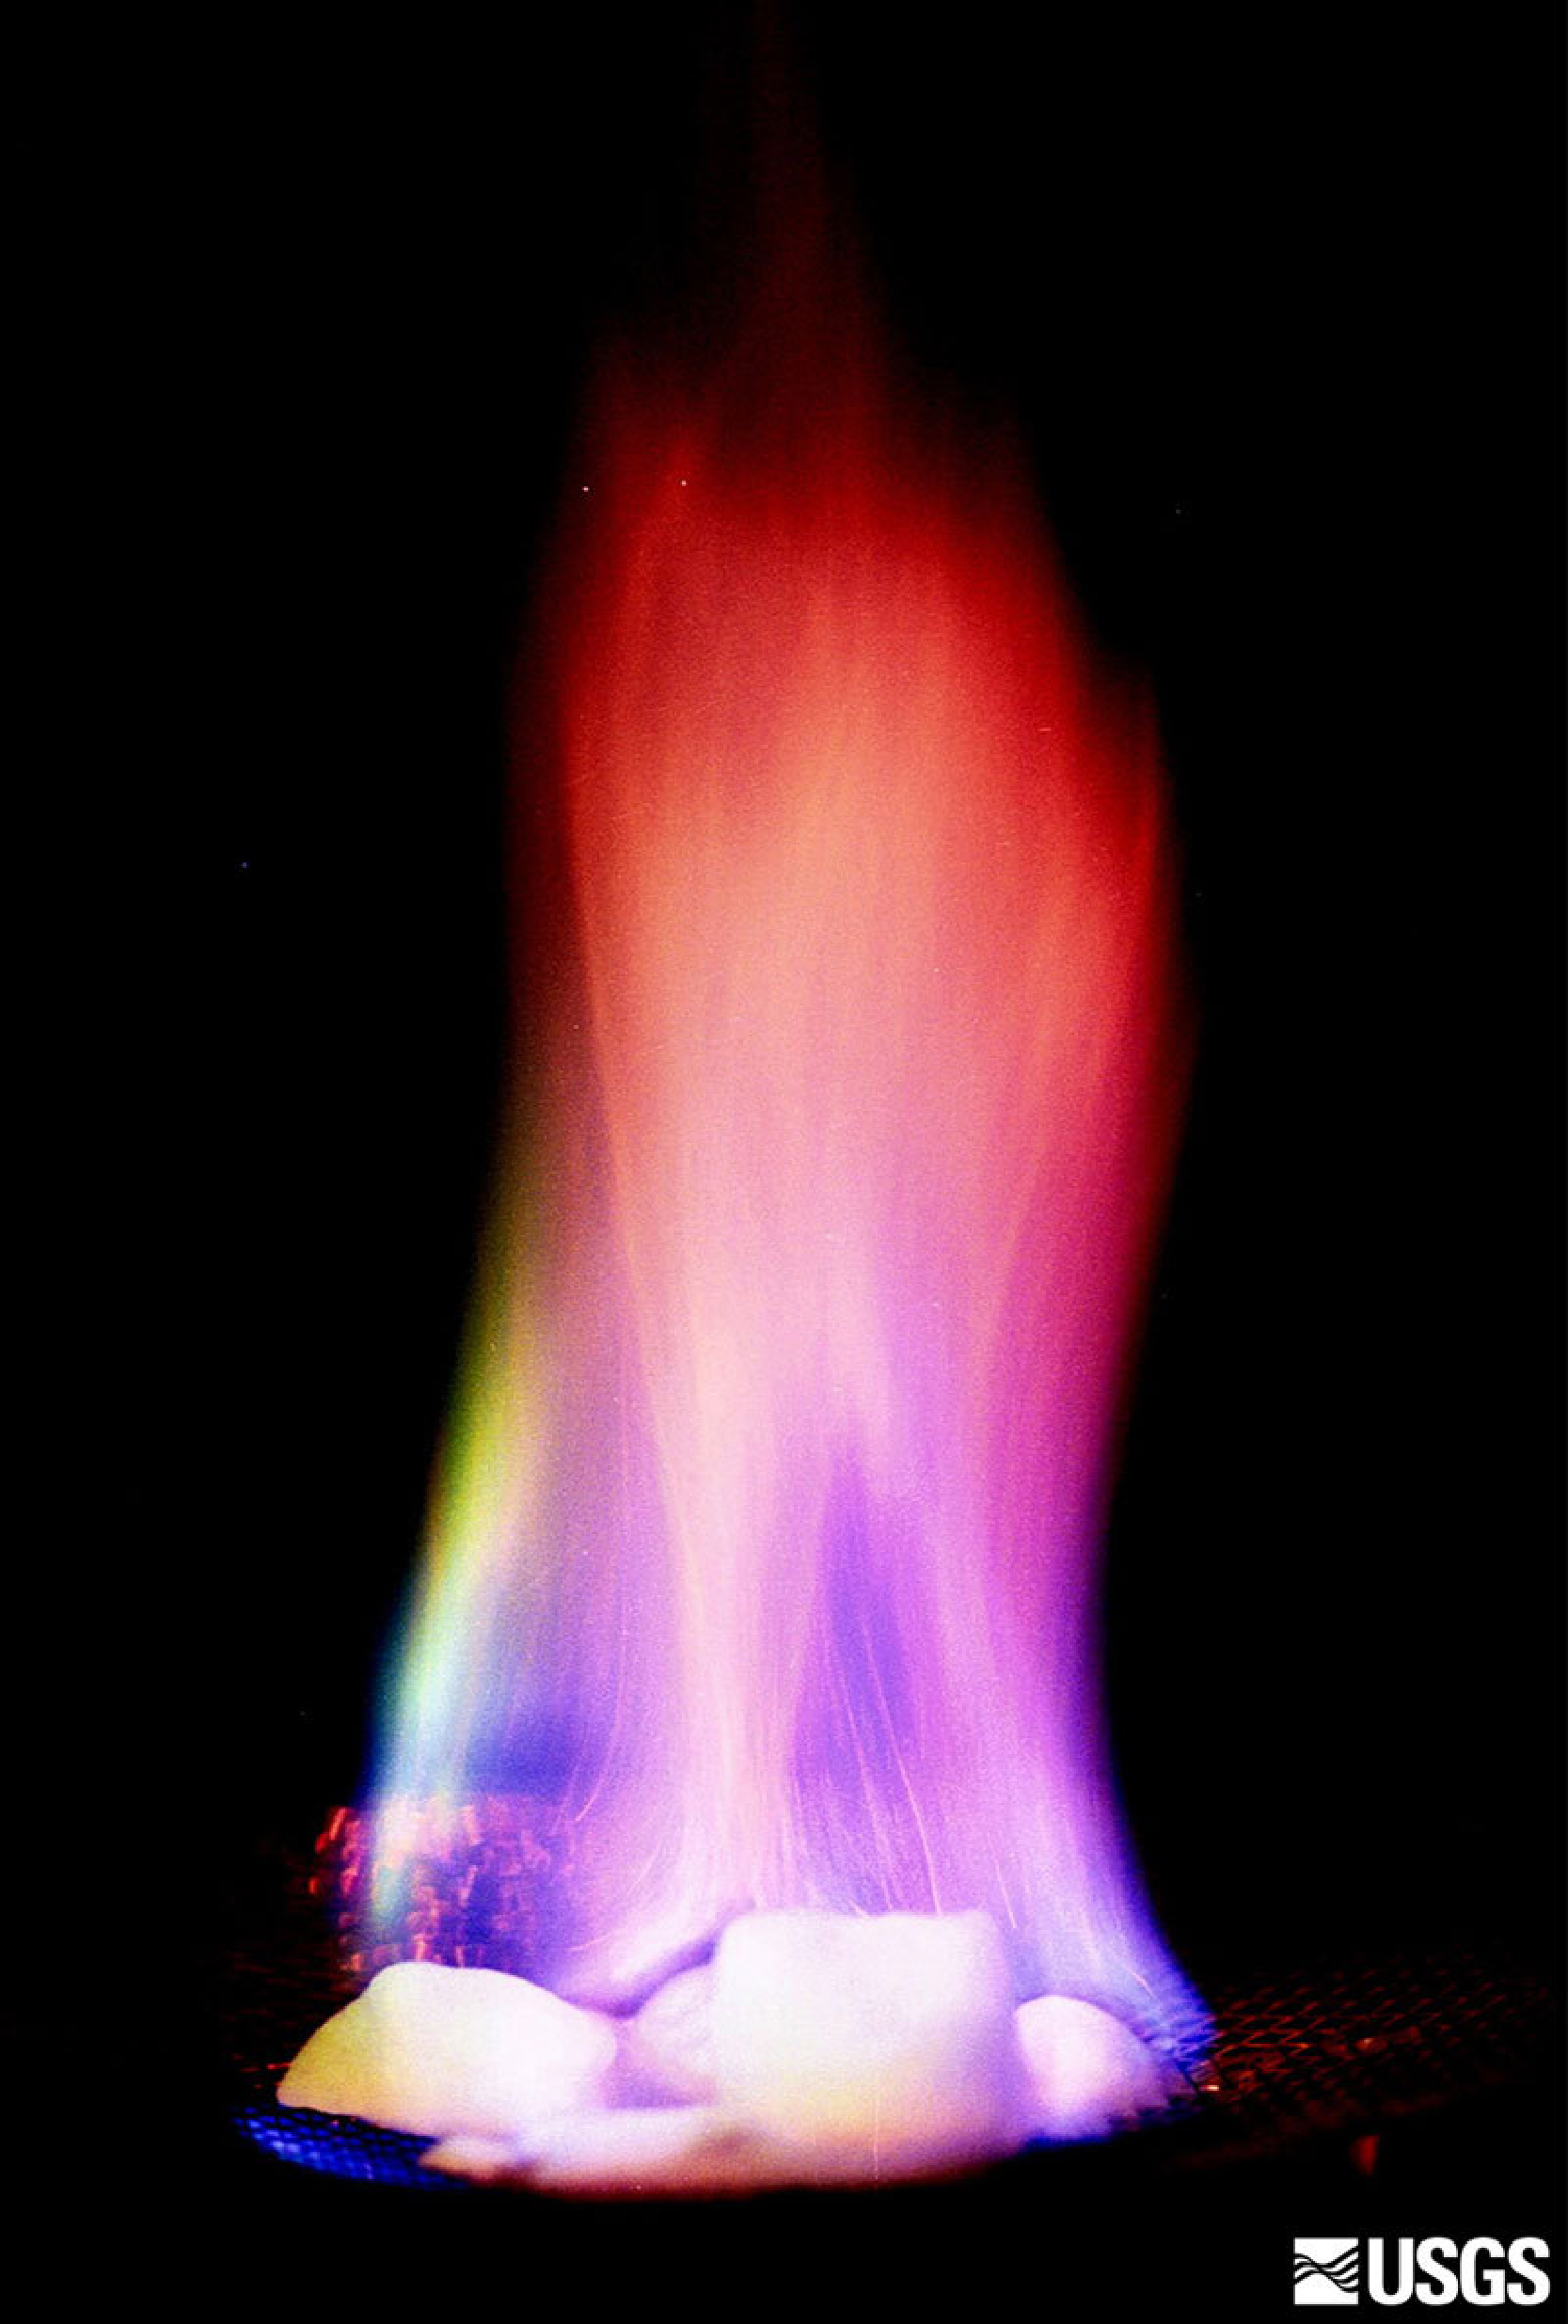
\includegraphics[width=0.8\textwidth]{../pictures/burning_hydrate.pdf}
\end{figure}

\column{0.5\textwidth}
\begin{itemize}
\item Et isliknende stoff som inneholder molekyler av stoffer som opptrer som gasser under vanlige forhold.
\item Vanligvis mener man metanhydrater når man sier gasshydrater.
\end{itemize}

\end{columns}
\myref{Figur: \textit{U.S. Geological Survey}}
\end{frame}

%\subsection{}
\begin{frame}
\frametitle{Bruksområder}
\begin{columns}
\column{0.3\textwidth}
\begin{itemize}
\item Energi (brenne metan)
\item CO$_2$-lagring
\end{itemize}
\column{0.7\textwidth}
\begin{figure}
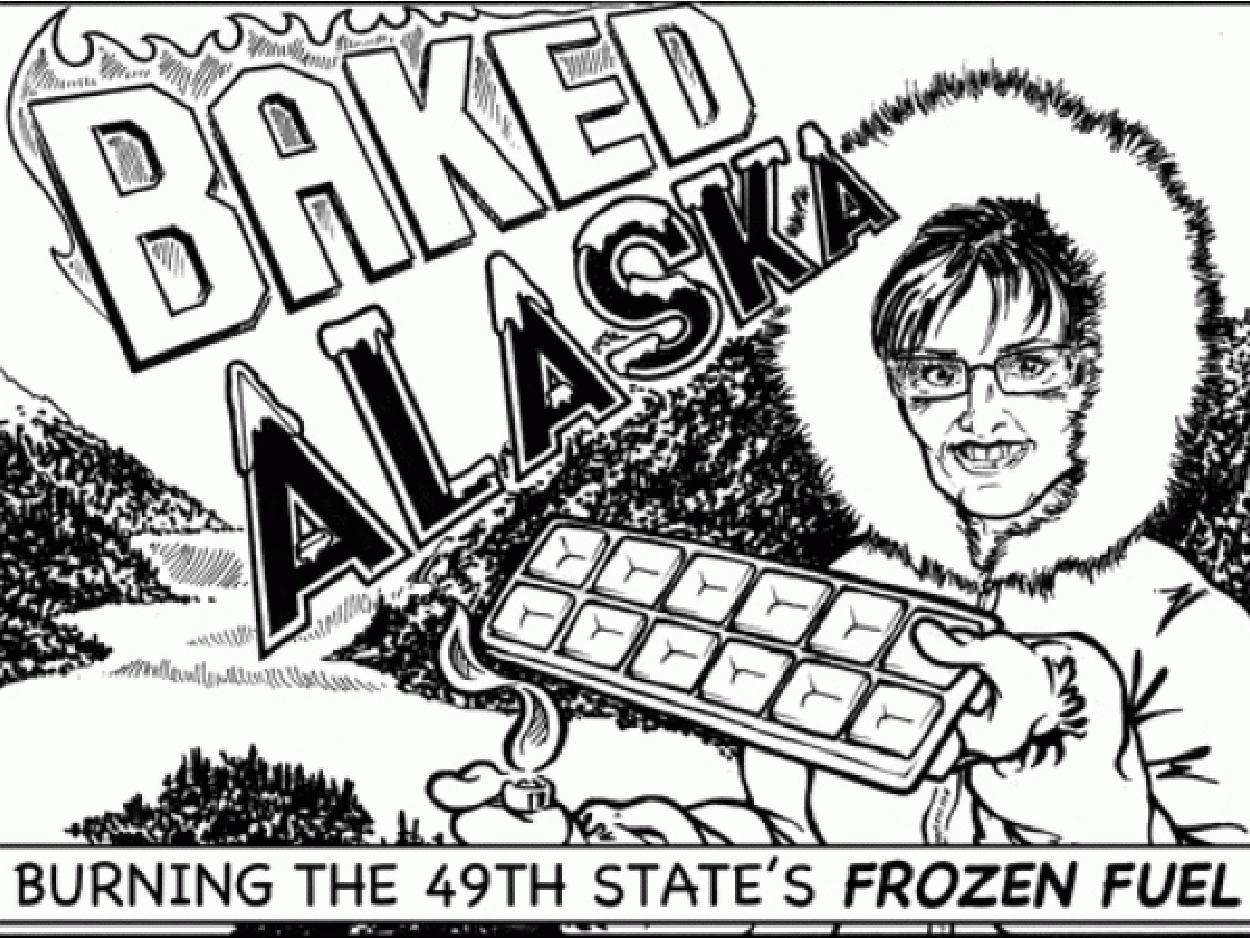
\includegraphics[width=0.9\textwidth]{../pictures/baked_alaska.pdf}
\end{figure}
\end{columns}
\end{frame}


%\subsection{}
\begin{frame}
\frametitle{Det ligger masse gasshydrater i havet, men sannsynligvis ikke så mye som man ofte blir fortalt..}

\begin{tikzpicture}[overlay]
\coordinate (x1) at ($(current page.center)-(0,1cm)$);
\only<1>{
\node[opacity=1.0] at (x1){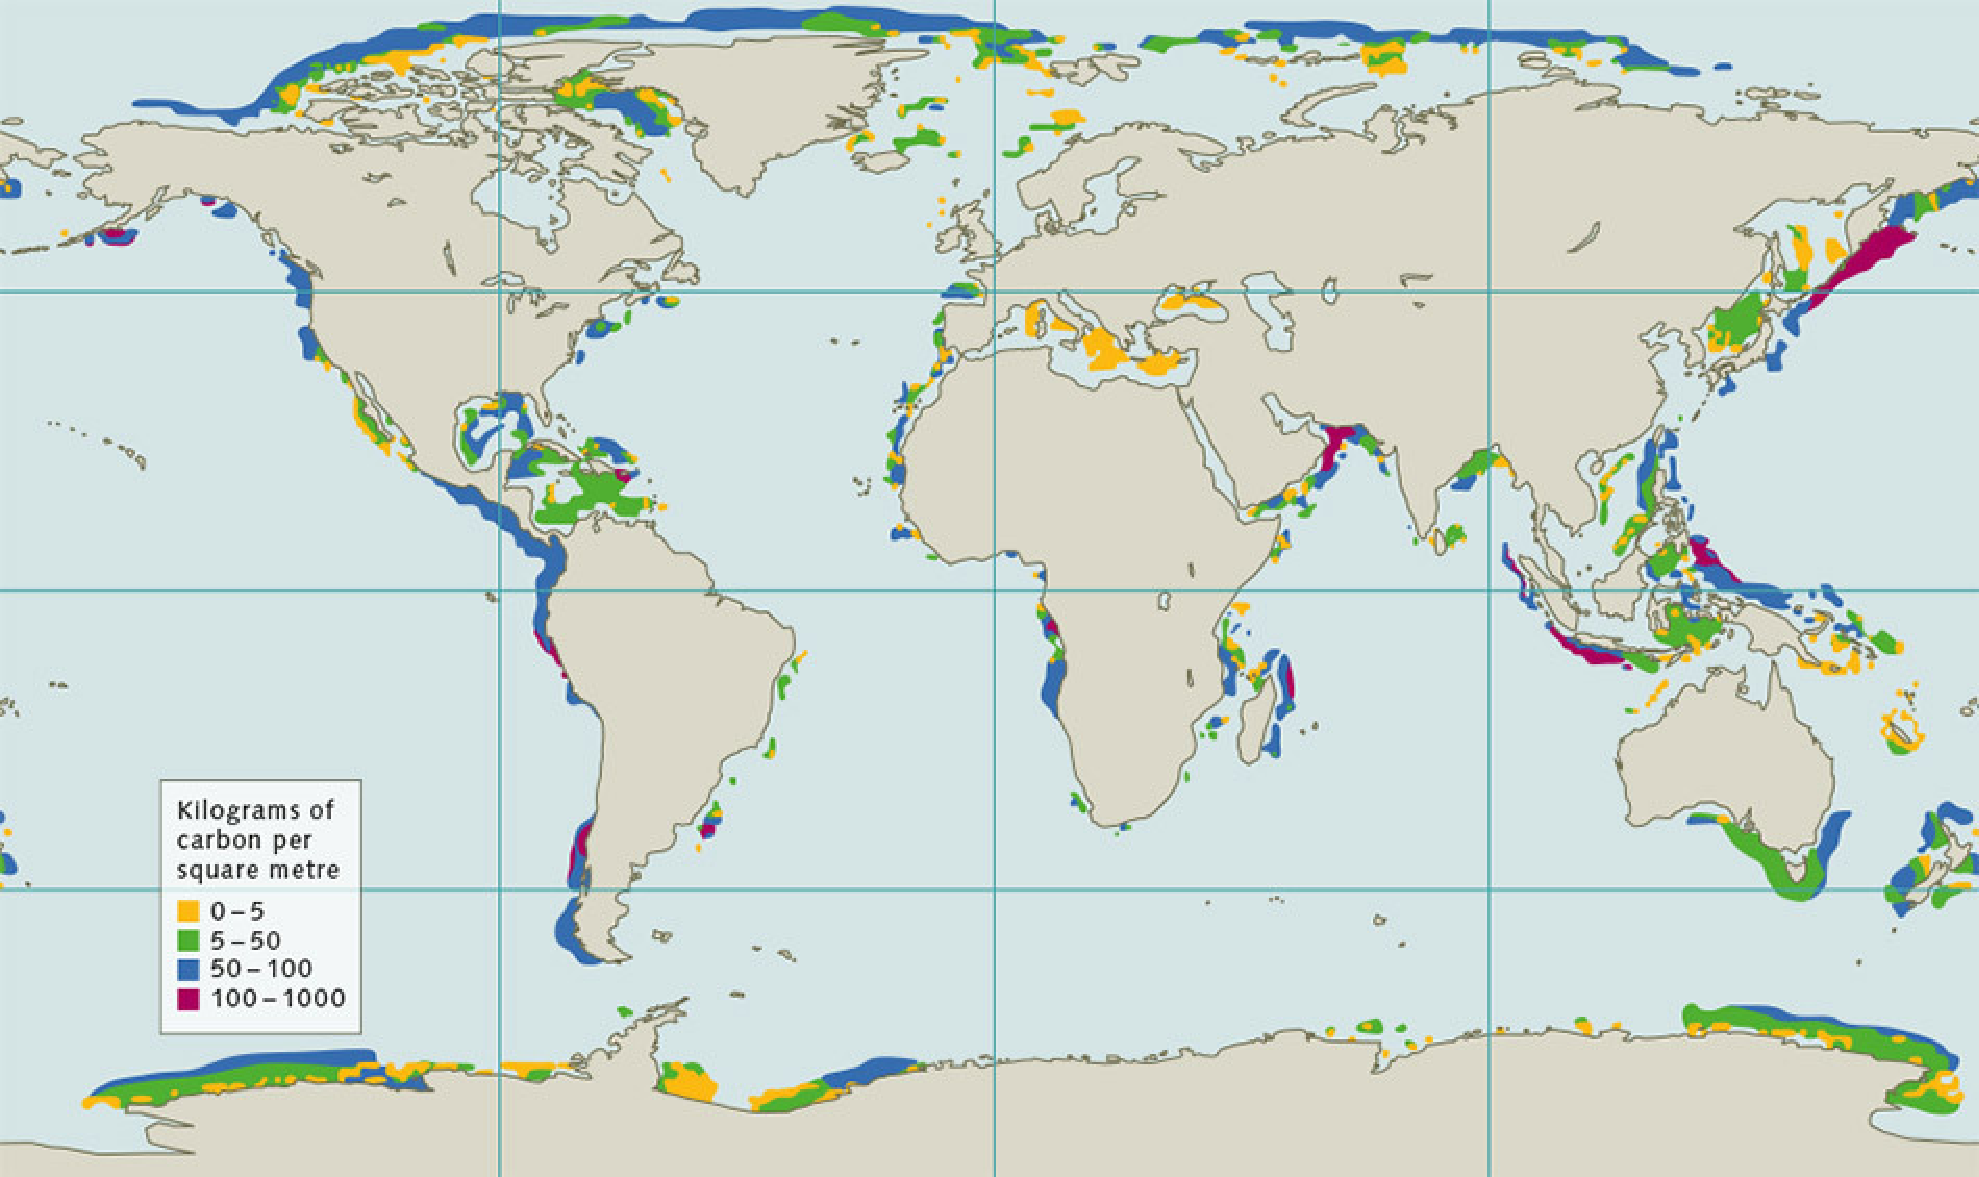
\includegraphics[width=\textwidth]{../pictures/hydrate_map_nice.pdf}};
}
\only<2>
{
\node[opacity=0.2](watermarkmap) at (x1){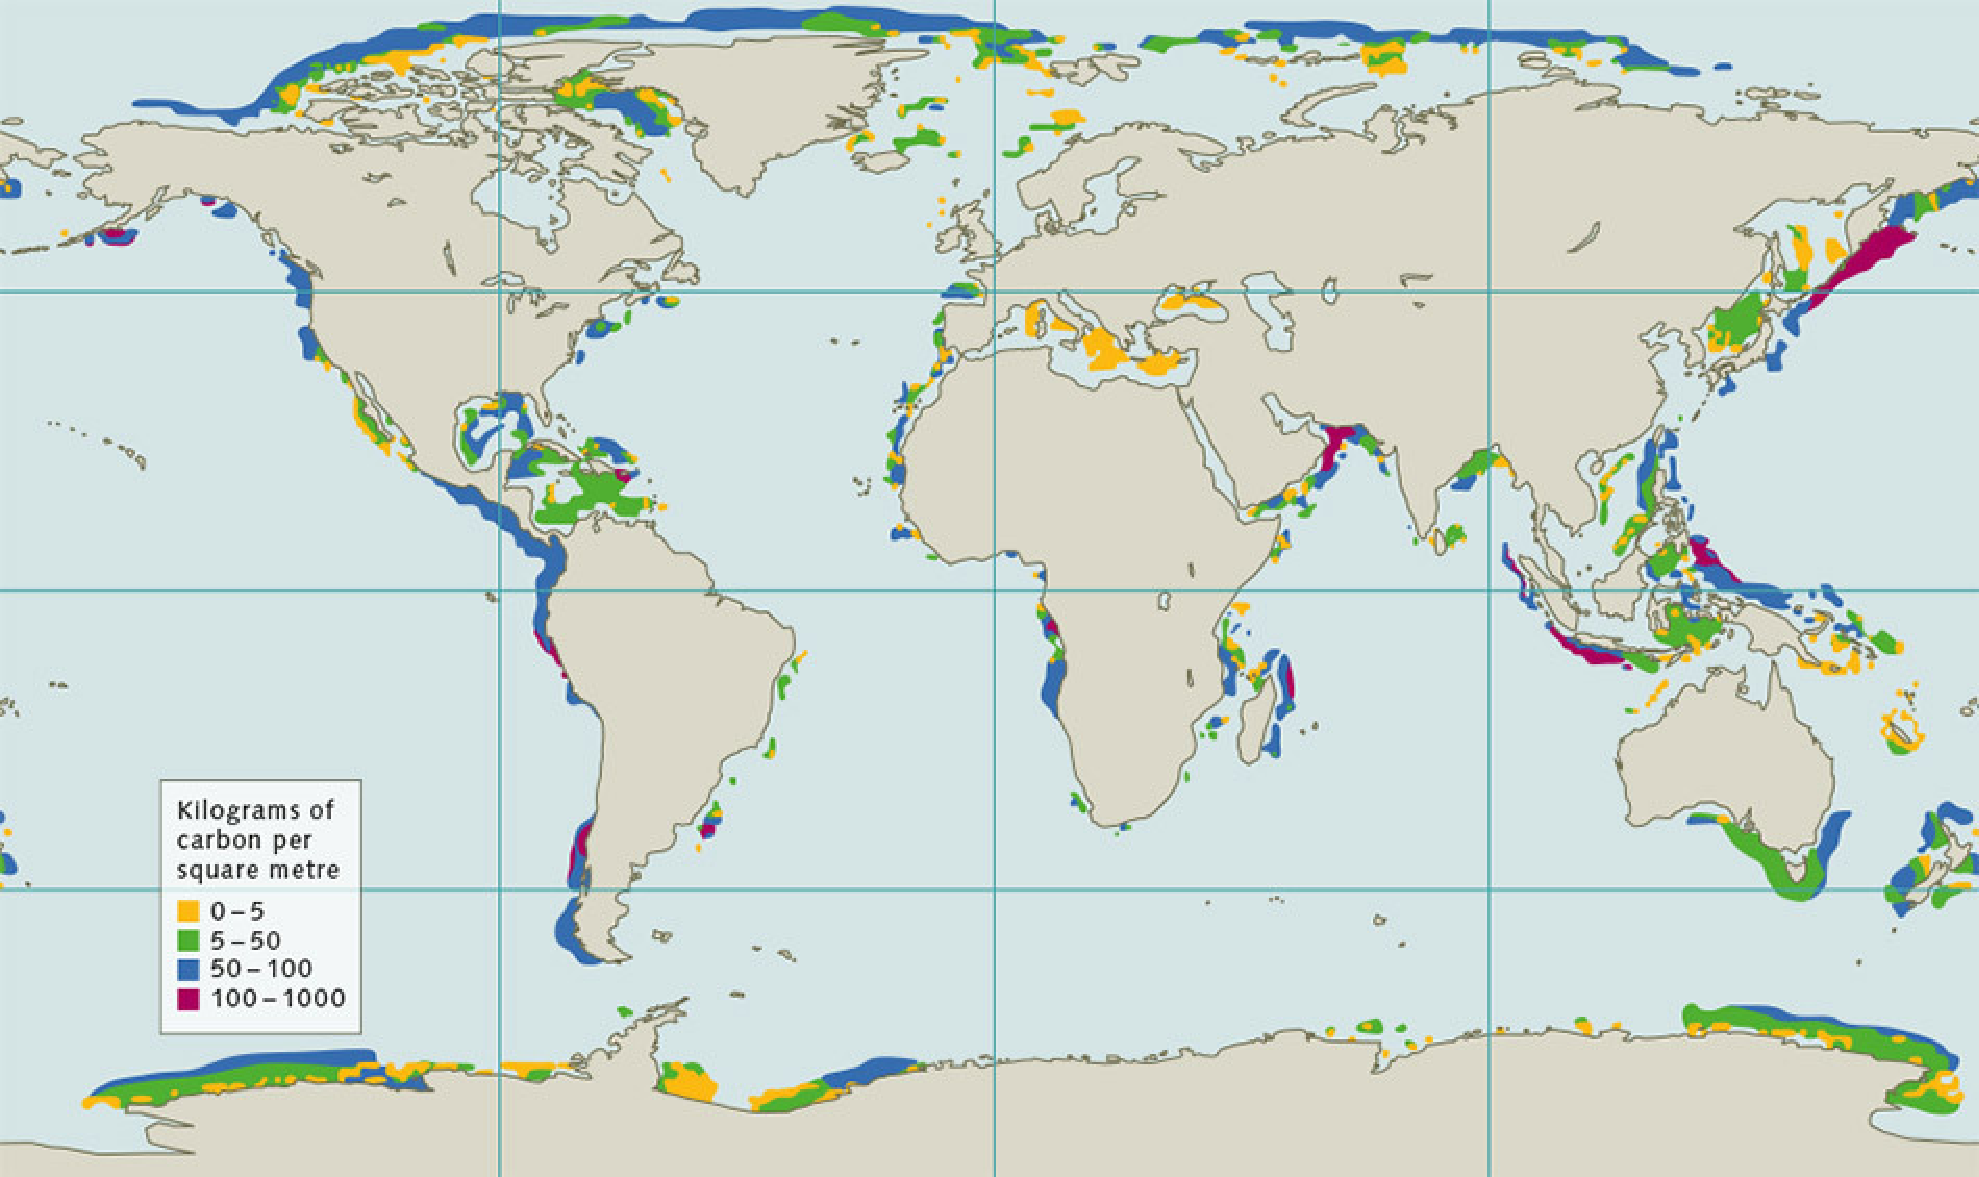
\includegraphics[width=\textwidth]{../pictures/hydrate_map_nice.pdf}};
\node[align=center] (text) at (x1) {Kartet viser ca 500 gigatonn med karbon lagret i gasshydrater. \\Det er mye. \\Vanlige estimater ligger mellom 500 og 2500 gigatonn. \\Høye estimater er $\sim$ 10 000 gigatonn. \\ \\Det 120 gigatonn karbon i kjente naturgassreservoarer.};
}
\end{tikzpicture}
\only<1-2>
{
\myref{Figur: \textit{The World Ocean Review, Marine Resources -- Opportunities and Risks, 2014}}
}

\only<3>
{
	\begin{figure}
		\centering
		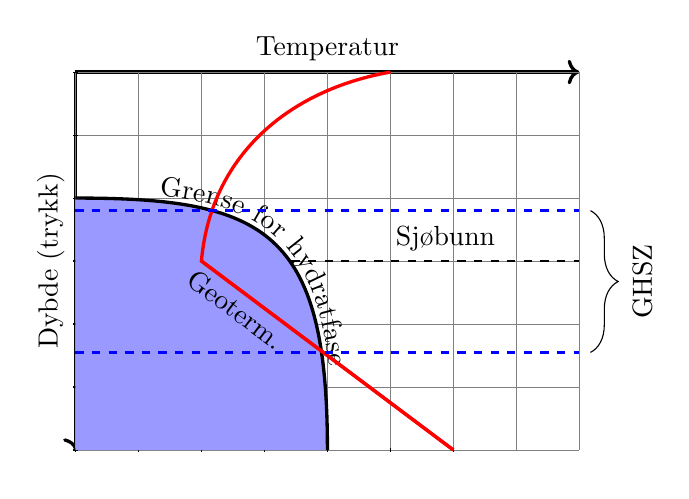
\begin{tikzpicture}[scale=0.8]
		\draw[very thick,->] (0,6) -- (8,6) node[midway, above] (temptext) {Temperatur};
		\draw[very thick,->] (0,6) -- (0,0) node[midway, above, rotate=90] (depthtext) {Dybde (trykk)};
		\draw[step=1cm,gray,very thin] (0,0) grid (8,6);
		\foreach \x in {0,1,2,3,4, 5, 6}
		    \draw (\x cm,1pt) -- (\x cm,-1pt) node[anchor=north] {};
		\foreach \y in {0,1,2,3,4, 5, 6}
		    \draw (1pt,\y cm) -- (-1pt,\y cm) node[anchor=east] {};
		\draw[name path=stability] (0, 4) .. controls (3.0, 4) and (4, 3.5) .. (4, 0); % Stability
		\draw[name path=watertemp] (5, 6) to [out=190, in=85] (2, 3.0) -- (6, 0) ; 
		\draw[dashed] (0, 3) -- (8, 3) node[above, xshift=-1.7cm] (textpermafrost) {Sjøbunn};
		\fill[blue!40!white!]
			(0, 4) .. controls (3.0, 4) and (4, 3.5) .. (4, 0) -- (0, 0) -- (0, 4);
		\draw[name path=stability, very thick, postaction={decorate, decoration={text along path, text align=center, raise=2pt, text={Grense for hydratfase}}}] (0, 4) .. controls (3.0, 4) and (4, 3.5) .. (4, 0); % Stability
		\draw[red, name path=geoterm, very thick, postaction={decorate, decoration={text along path, text align=left, raise=-10pt, text={Geoterm.}}}](2, 3.0) -- (6, 0); % Geoterm parmafrost
		\draw[red, very thick] (5, 6) to [out=190, in=85] (2, 3.0) -- (6, 0);
		\draw[dashed, very thick, blue] (0, 3.8) -- (8, 3.8);
		\draw[dashed, very thick, blue] (0, 1.55) -- (8, 1.55);
		\draw [decorate,decoration={brace,amplitude=10pt,mirror,raise=4pt},yshift=0pt]
		(8 ,1.55) -- (8, 3.8) node [black,midway,xshift=0.8cm, rotate=90] {GHSZ};
		\end{tikzpicture}
	\end{figure}
}
\end{frame}


%\subsection{}
\begin{frame}
\frametitle{Risiko}
\begin{columns}[T]
\column{0.5\textwidth}
\begin{block}{Operasjonell}
\begin{itemize}
\item Tette rør
\end{itemize}
\end{block}

\begin{figure}
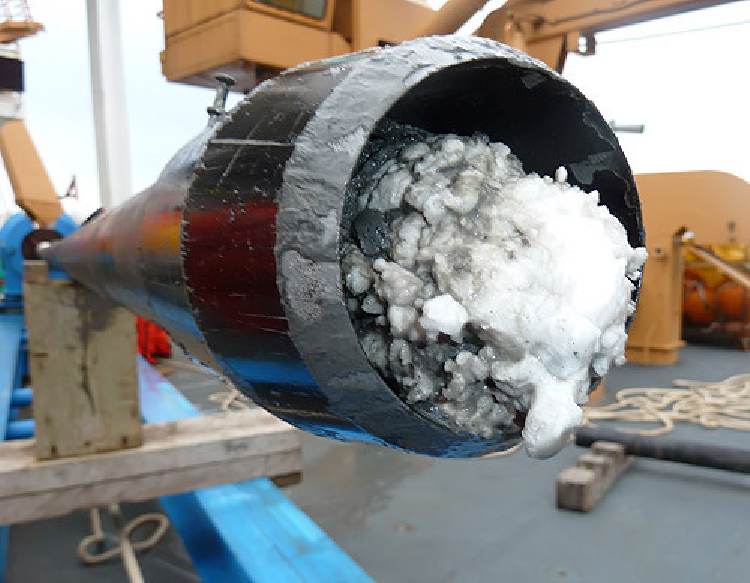
\includegraphics[width=0.8\textwidth]{../pictures/pipe_plug.pdf}
\end{figure}

\column{0.5\textwidth}
\begin{block}{Geologisk}
\begin{itemize}
\item Sedimentskred
\item \emph{the clathrate gun hypothesis}
\end{itemize}
\end{block}
\end{columns}
\myref{Figur: https://www.youtube.com/watch?v=nUluhIa-hzA}
\end{frame}

\begin{frame}
\frametitle{Overordnet mål: Utvinne metan fra gasshydrater, og lagre CO$_2$}
\begin{tikzpicture}[overlay, shift={($(current page.center)-(0,0.7)$)}]
\node (pic) at (0, 0) {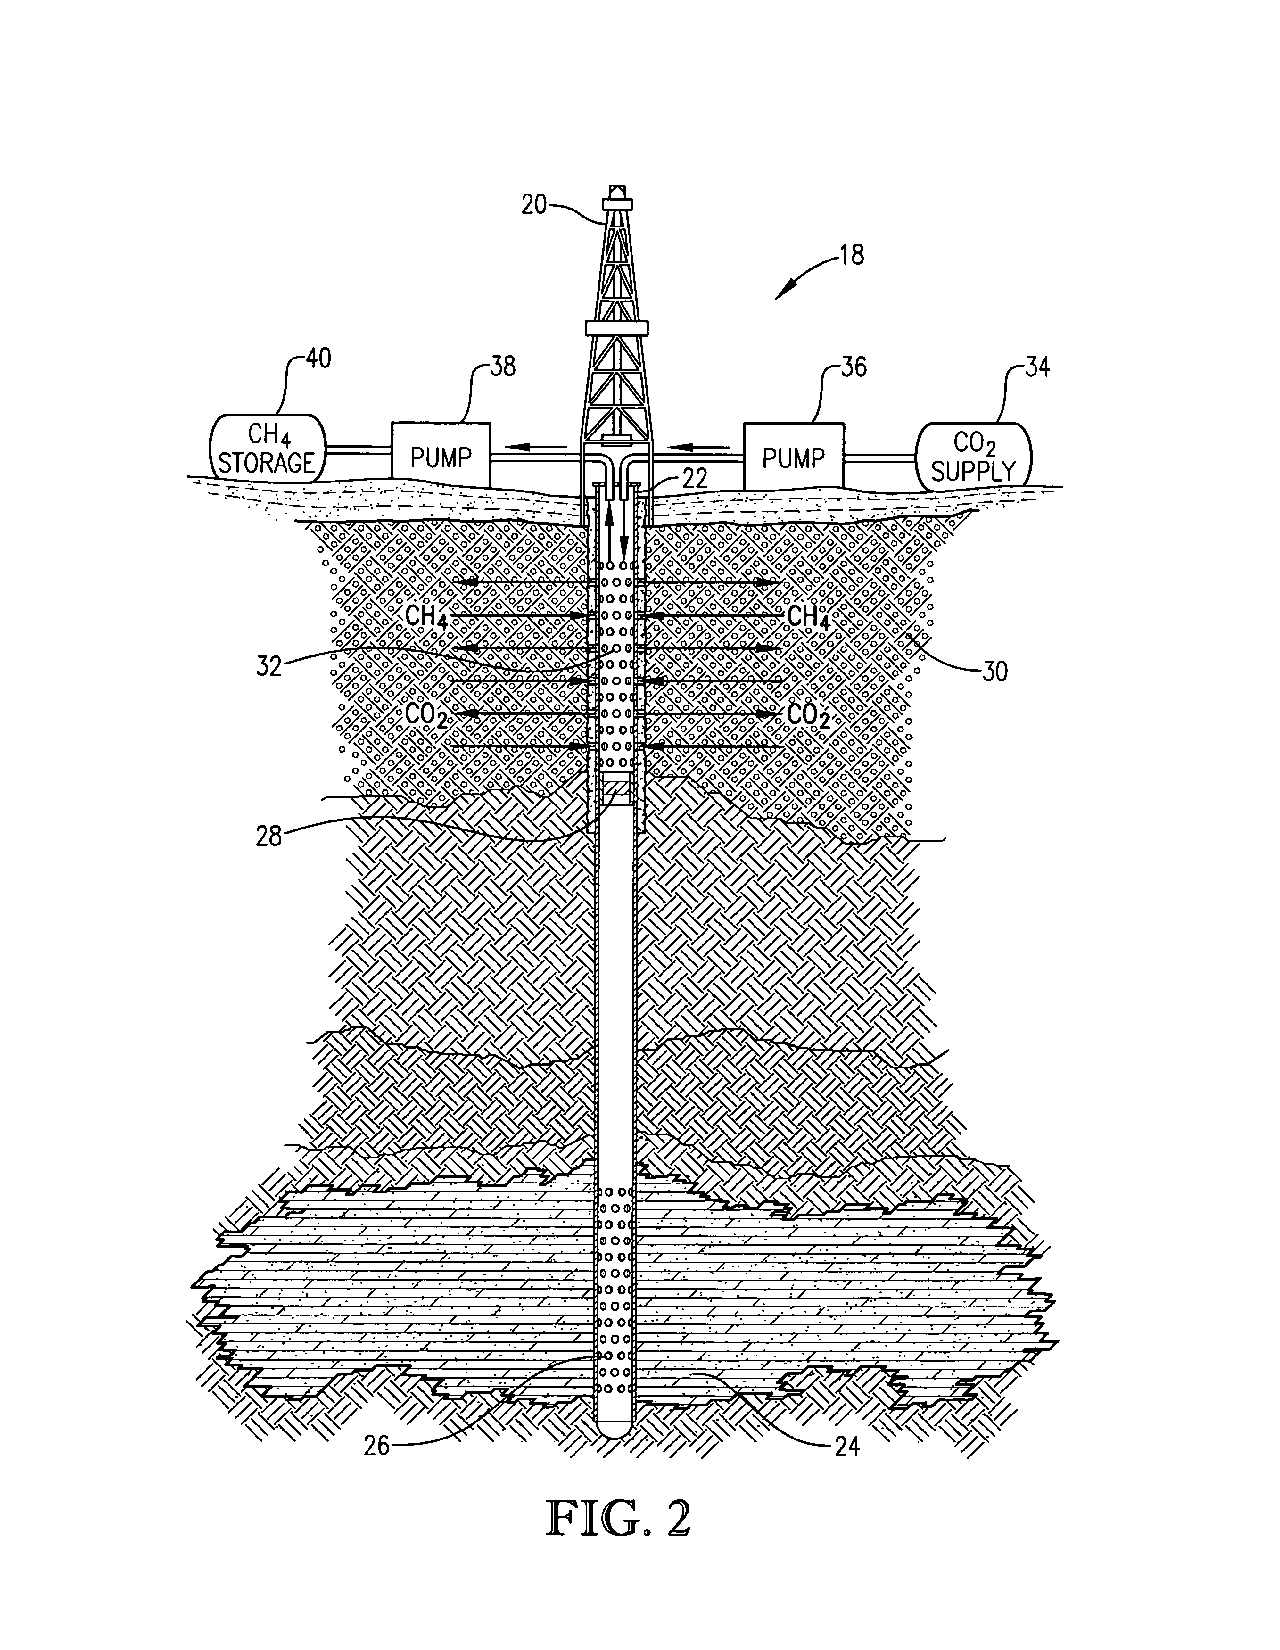
\includegraphics[height=0.87\textheight]{../pictures/utvinning.pdf}};
\end{tikzpicture}
\myref{Figur: US patent 7,222,637 B2}
\end{frame}


\begin{frame}
\frametitle{Hva lurer vi på akkurat nå?}
Hvordan sprekker i gasshydrater bidrar til å oppløse hydratet.
\begin{columns}[T]
\column{0.5\textwidth}
\begin{block}{Materialegenskaper}
\begin{itemize}
\item Hva er bruddstyrken?
\item Er gasshydratet spøtt eller duktilt?
\item Hvor mye metan frigjøres ved oppsprekking?
\item Hva er bruddmekanismen?
\end{itemize}
\end{block}
\column{0.5\textwidth}
\begin{block}{Simuleringsteknisk}
\begin{itemize}
\item Hvilke interaksjonspotensialer er best?
\item Hvordan bør man utløse sprekker?
\end{itemize}
\end{block}
\end{columns}
\end{frame}

\section{Modellering og simulering (med resultater)}

\subsection{}
%%%%%%%%%%%%%%%%%%
%\begin{comment}
%%%%%%%%%%%%%%%%%
\begin{frame}
\frametitle{Molekylærdynamikk: Tidsutvikle et system av punktpartikler som styres av Newtons 2. lov, $\mathbf{F} = m\ddot{\mathbf{r}}$}
\begin{columns}
\column{0.4\textwidth}
\pgfplotsset{width=5cm, compat=1.8}
\only<1-3>
{
\begin{figure}
\begin{tikzpicture}[baseline]
\begin{axis}[
	xmin=0,
	xtick={0,5,10},
	ytick=\empty,
	xlabel={$r$ [\AA]},
	ylabel={$U$ [arb. enhet]},
	title=Potensialer:,
	]
\addplot[
	red,
	domain=3.5:10,
	samples=100,
]
{(1/((x/3.73)^12)-1/((x/3.73)^6))};
\addplot[
	blue,
	domain=2.0:10,
	samples=100
]
{1/x};
\end{axis}
\draw[black, <->] (0, 0.8) -- node[above] (n1) {$\sigma$} (1.17, 0.8) ;
\end{tikzpicture}
\end{figure}
}
\only<4->
{
	\zerodisplayskips
	\begin{block}{\textcolor{red}{Lennard--Jones-potensialet}}
	\vspace{-4mm}
	\begin{equation*}
	U_1 = 4\epsilon\left[\left(\frac{\sigma}{r}\right)^{12}-\left(\frac{\sigma}{r}\right)^6\right]
	\end{equation*}
	\end{block}
	\begin{block}{\textcolor{blue}{Coulomb-potensialet}}
	\vspace{-4mm}
	\begin{equation*}
	U_2 = k\frac{q_aq_b}{r}
	\end{equation*}
	\end{block}
	\begin{block}{\textcolor{gray}{Kraftberegning}}
	\vspace{-4mm}
	\begin{equation*}
	\mathbf{F} = -\nabla U
	\end{equation*}
	\end{block}
}
\column{0.5\textwidth}
\only<1>
{
\begin{tikzpicture}[remember picture,overlay]
  \tikzset{shift={(current page.center)},yshift=-4cm}
\draw[blue!40!white] (0, 0) rectangle (5, 6);
\node (title) at (2.5, 6.3) {Partikler med posisjoner og hastigheter};
\pgfmathsetseed{1138}
\foreach \i in {1, 2, ..., 100}
{
	\pgfmathrandominteger{\x}{0}{500}
	\pgfmathrandominteger{\y}{0}{600}
	\pgfmathrandominteger{\xsh}{0}{50}
	\pgfmathrandominteger{\ysh}{0}{60}
	\pgfmathrandominteger{\xsi}{0}{50}
	\pgfmathrandominteger{\ysi}{0}{60}
	\filldraw [red] (\x/100, \y/100) circle (1pt);
}
\end{tikzpicture}
}
\only<2>
{
\begin{tikzpicture}[remember picture,overlay]
  \tikzset{shift={(current page.center)},yshift=-4cm}
\draw[blue!40!white] (0, 0) rectangle (5, 6);
\node (title) at (2.5, 6.3) {Partikler med posisjoner og hastigheter};
\pgfmathsetseed{1138}
\foreach \i in {1, 2, ..., 100}
{
	\pgfmathrandominteger{\x}{0}{500}
	\pgfmathrandominteger{\y}{0}{600}
	\pgfmathrandominteger{\xsh}{-5}{5}
	\pgfmathrandominteger{\ysh}{-5}{5}
	\pgfmathrandominteger{\xsi}{0}{50}
	\pgfmathrandominteger{\ysi}{0}{60}
	\FPeval{\resultx}{clip(\x+\xsh)}
	\FPeval{\resulty}{clip(\y+\ysh)}
	\filldraw [gray!40!white] (\x/100, \y/100) circle (1pt);
	\filldraw [red] (\resultx/100, \resulty/100) circle (1pt);	
}
\end{tikzpicture}
}
\only<3->
{
\begin{tikzpicture}[remember picture,overlay]
  \tikzset{shift={(current page.center)},yshift=-4cm}
\draw[blue!40!white] (0, 0) rectangle (5, 6);
\node (title) at (2.5, 6.3) {Partikler med posisjoner og hastigheter};
\pgfmathsetseed{1138}
\foreach \i in {1, 2, ..., 100}
{
	\pgfmathrandominteger{\x}{0}{500}
	\pgfmathrandominteger{\y}{0}{600}
	\pgfmathrandominteger{\xsh}{-5}{5}
	\pgfmathrandominteger{\ysh}{-5}{5}
	\pgfmathrandominteger{\xsi}{-5}{5}
	\pgfmathrandominteger{\ysi}{-5}{5}
	\FPeval{\resultx}{clip(\x+\xsh)}
	\FPeval{\resulty}{clip(\y+\ysh)}
	\FPeval{\resultxi}{clip(\x+2*\xsh+\xsi)}
	\FPeval{\resultyi}{clip(\y+2*\ysh+\ysi)}
	\filldraw [gray!40!white] (\x/100, \y/100) circle (1pt);
	\filldraw [gray!40!white] (\resultx/100, \resulty/100) circle (1pt);
	\filldraw [red] (\resultxi/100, \resultyi/100) circle (1pt);	
}
\end{tikzpicture}
}
\end{columns}
\end{frame}


%\subsection{}
\begin{frame}
\frametitle{TIP4P/ICE + UAM (vann og metan)}
\only<1>
{
\begin{tikzpicture}[remember picture,overlay]
\tikzset{shift={(current page.center)},yshift=-1cm, xshift=-2cm}
\filldraw (0, 0) [green] circle [radius=1.0];
\draw (0, 0) [green!60!black] circle [radius=3.73];
\fill [violet, shift={(0, 0)}] (0, 0) circle [radius=0.1];

\filldraw [red!60!black,shift={(6, 2)}, rotate=210] (0, 0) circle [radius=0.7] node (o1) {} [gray!40!white] (-52.5:0.95) circle [radius=0.4] node (h1) [black]{+} (52.5:0.95) circle [radius=0.4] node (h2) [black] {+};
\draw (6, 2) [red] circle [radius=3.16];
\fill [red, shift={(6, 2)}] (0, 0) circle [radius=0.7] node[circle, draw, fill=red!20!white] (m2) at (210:0.38) {--};
\fill [violet, shift={(6, 2)}] (0, 0) circle [radius=0.1];

\filldraw [red!60!black,shift={(5, -2)}, rotate=120] (0, 0) circle [radius=0.7] node (o2) {} [gray!40!white] (-52.5:0.95) circle [radius=0.4] node (h21) [black]{+} (52.5:0.95) circle [radius=0.4] node (h22) [black]{+};
\draw (5, -2) [red] circle [radius=3.16];
\fill [red, shift={(5, -2)}] (0, 0) circle [radius=0.7] node[circle, draw, fill=red!20!white] (m2) at (120:0.38) {--};
\fill [violet, shift={(5, -2)}] (0, 0) circle [radius=0.1];

\fill[violet] (-4, 4) circle[radius=0.1] node[xshift=69] (ljdef) {Lennard--Jones-sentrum};

\fill[red!20!white] (-4, 3.3) circle[radius=0.3] node (ljdef) [red] {--} node [xshift=51] {Negativ ladning};

\fill[gray!40!white] (-4, 2.6) circle[radius=0.3] node (ljdef) [black] {+} node [xshift=49] {Positiv ladning};

%\draw [red!60!black, shift={(6, 2)}] (0, 0) circle [radius=0.7] node (o1) {} [gray] (-52.5:1.0) circle [radius=0.4] node(h1) {} (52.5:1.0) circle [radius=0.4] node (h2) {};

%\draw (6, 2) [blue] node[rotate=-30] (h2o1) {\chemfig{O(-[:-142]H)(-[:-38]H)(-[:270, 0.5]M)}};
%\draw (6, -2) [blue] node[rotate=-130] (h2o2) {\chemfig{O(-[:-142]H)(-[:-38]H)(-[:270, 0.5]M)}};
%\path [violet, draw, <->, very thick]  (ch41.center) -- node[above] {$LJ$} ($(h2o1.north)+(-0.2,-0.2)$);
%\path [violet, draw, <->, very thick]  (ch41.center) -- node[below] {$LJ$} (h2o2.north);
%\path [violet, draw, <->, very thick]  (h2o2.north) -- node[right] {$LJ$} (h2o1.north);
\end{tikzpicture}
}
\only<2>
{
	\begin{figure}
		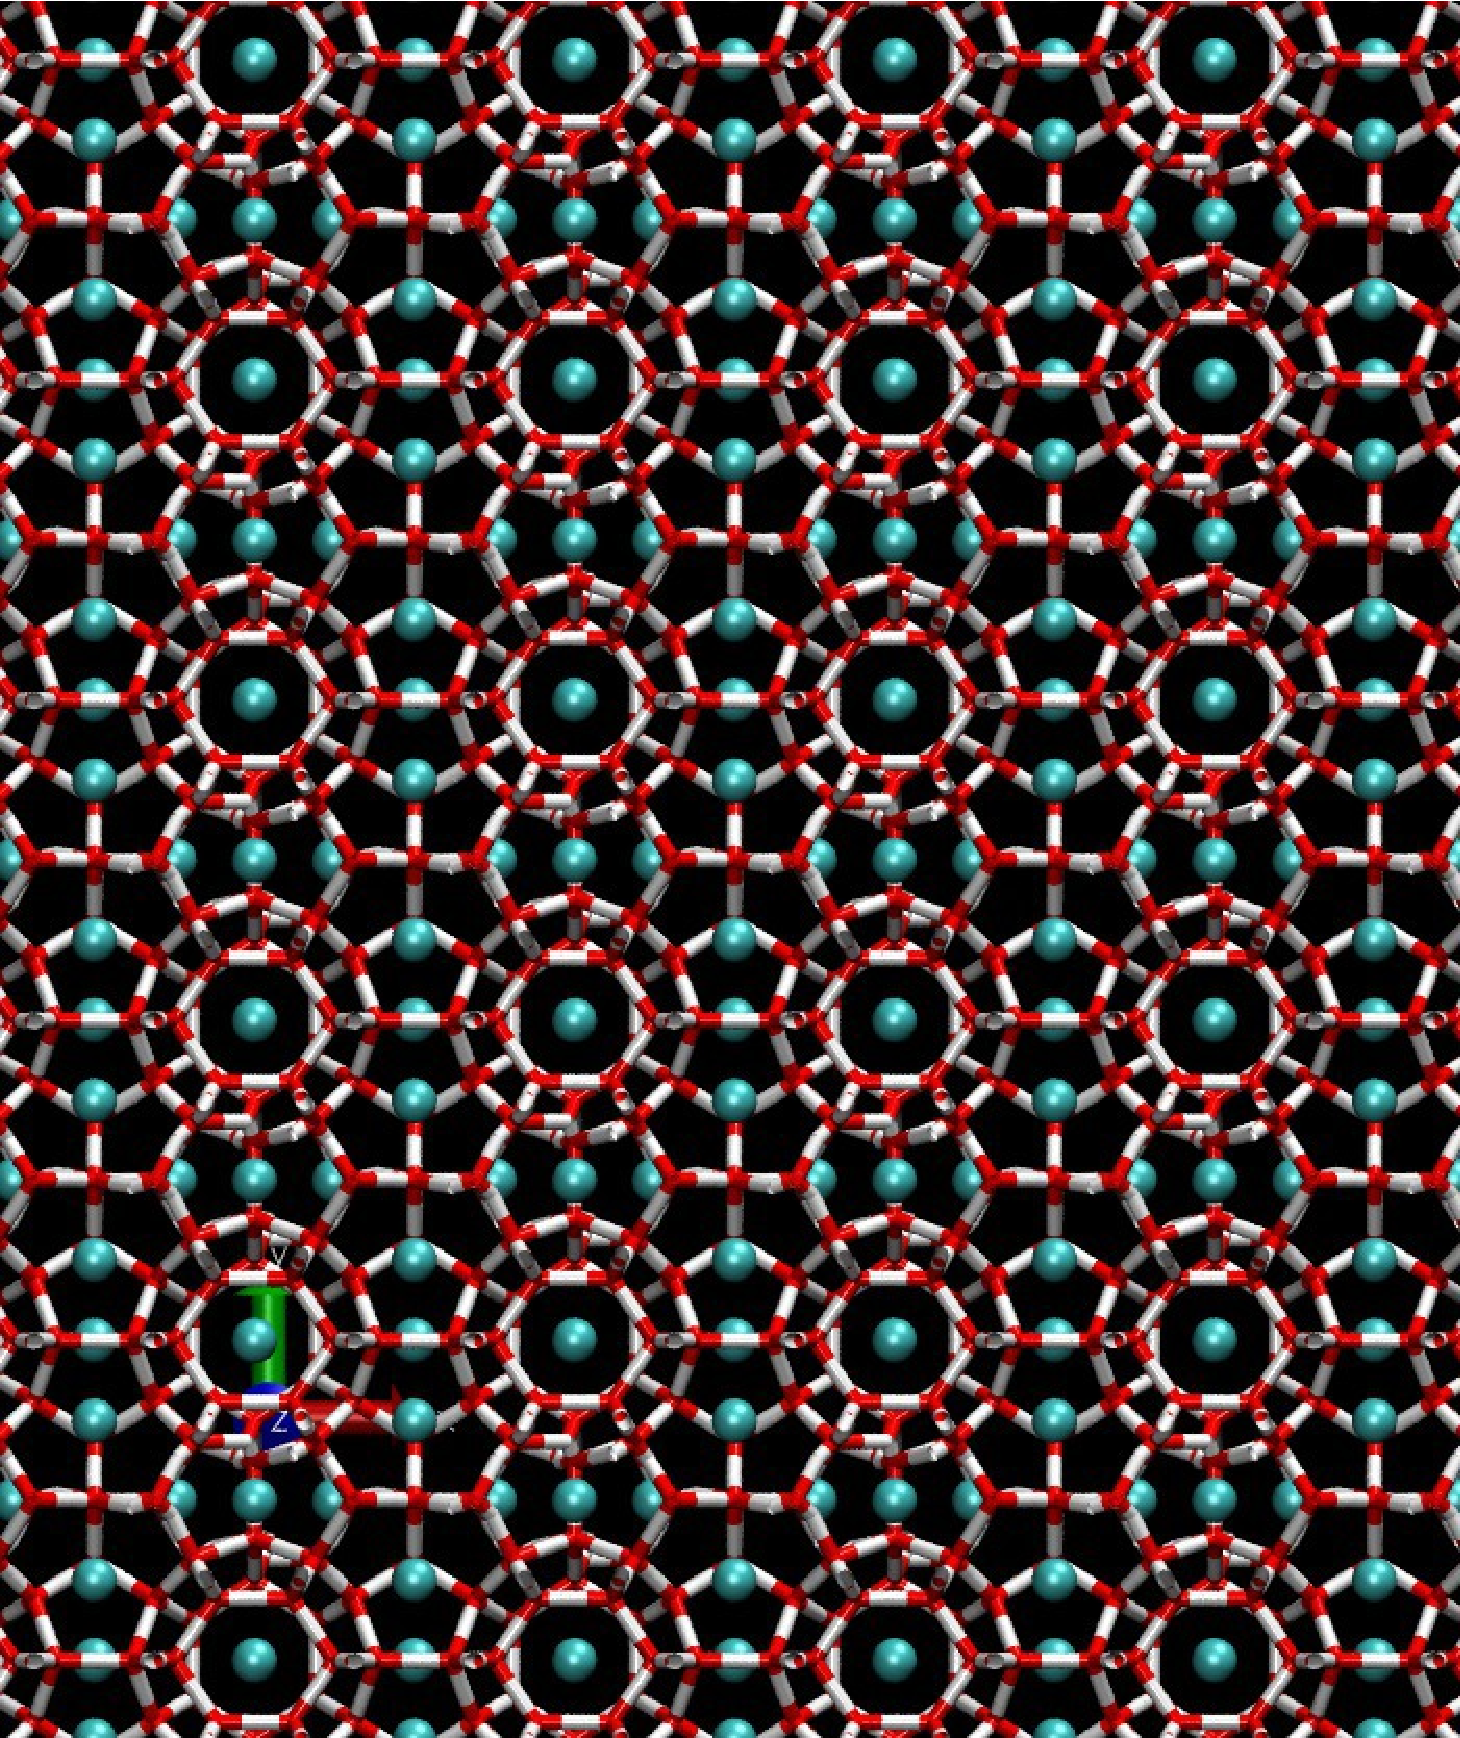
\includegraphics[height=0.8\textheight]{../snapshots/bulk_hydrate.pdf}
	\end{figure}
}
\end{frame}
%\end{comment}

\begin{frame}
\frametitle{Simulert system for elastiske egenskaper}
\only<1>
{
\begin{tikzpicture}[overlay, shift={($(current page.center)-(2.5,3.5)$)}]
\filldraw[fill=blue!40!white] (0, 0) rectangle (5, 5);
\foreach \i in {0.5, 1.5, 2.5, 3.5, 4.5}
{
	\draw[thick, ->] (5, \i) -- (6, \i);
	\draw[thick, ->] (0, \i) -- (-1, \i);
}
\draw [decorate,decoration={brace,amplitude=4pt,mirror,raise=4pt},yshift=0pt]
		(5, 5) -- (0, 5) node [black,midway,yshift=0.6cm, rotate=0] {$l_0$};
\end{tikzpicture}
}
\only<2>
{
\begin{tikzpicture}[overlay, shift={($(current page.center)-(2.5,3.5)$)}]
\filldraw[fill=blue!40!white, opacity=0.4] (0, 0) rectangle (5, 5);
\filldraw[fill=blue!40!white] (-1, 0.5) rectangle (6, 4.5);
\foreach \i in {0.9, 1.7, 2.5, 3.3, 4.1}
{
	\draw[thick, ->] (6, \i) -- (7, \i);
	\draw[thick, ->] (-1, \i) -- (-2, \i);
}
\draw [decorate,decoration={brace,amplitude=4pt,mirror,raise=2pt},yshift=0pt]
		(-1, 4.5) -- (0, 4.5) node [black,midway,yshift=-0.6cm, rotate=0] {$\frac{\Delta x}{2}$};
\draw [decorate,decoration={brace,amplitude=4pt,mirror,raise=2pt},yshift=0pt]
		(0, 4.5) -- (0, 5) node [black,midway,xshift=0.6cm, rotate=0] {$\frac{\Delta y}{2}$};
\end{tikzpicture}
}

\only<3>
{
Beregner Youngs modul og Poissonforholdet basert på de forrige figurene:

\begin{columns}[T]

\column{0.5\textwidth}
\begin{block}{Youngs modul}
\begin{equation*}
 E=\frac{F_x l_0}{A\Delta x} = \frac{\sigma_x}{\epsilon_x}
\end{equation*}
\end{block}

\column{0.5\textwidth}
\begin{block}{Poissonforholdet}
\begin{equation*}
\nu = -\frac{\Delta y}{\Delta x}
\end{equation*}
\end{block}
\end{columns}
}
\end{frame}

\begin{frame}
\frametitle{Elastiske egenskaper}
\only<1>
{
	\begin{columns}
	\column{0.7\textwidth}
	\begin{figure}
		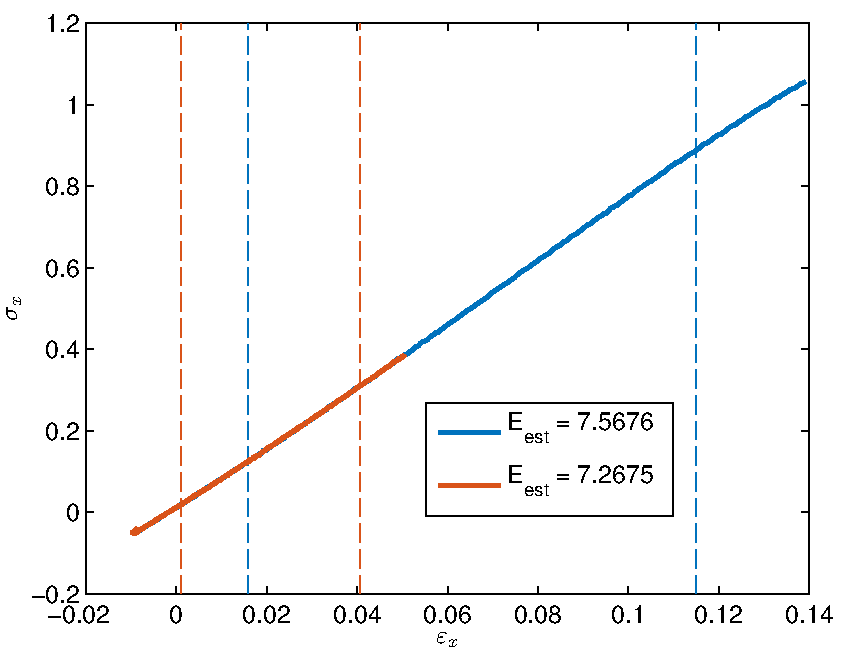
\includegraphics[width=\textwidth]{../figures/thesis/stress_strain_11_11_11_tip4p_ice_uam.pdf}
	\end{figure}
	\column{0.3\textwidth}
	Youngs modul er omtrent 7.1 GPa.\\
	\vspace{3mm}
	Det ser bra ut. (Exp $\approx 7.8$ GPa).
	\vspace{3mm}
	Til sammenlikning: PMMA har $\approx 3$ GPa.
	\end{columns}
}
\only<2>
{
	\begin{columns}
	\column{0.7\textwidth}
	\begin{figure}
		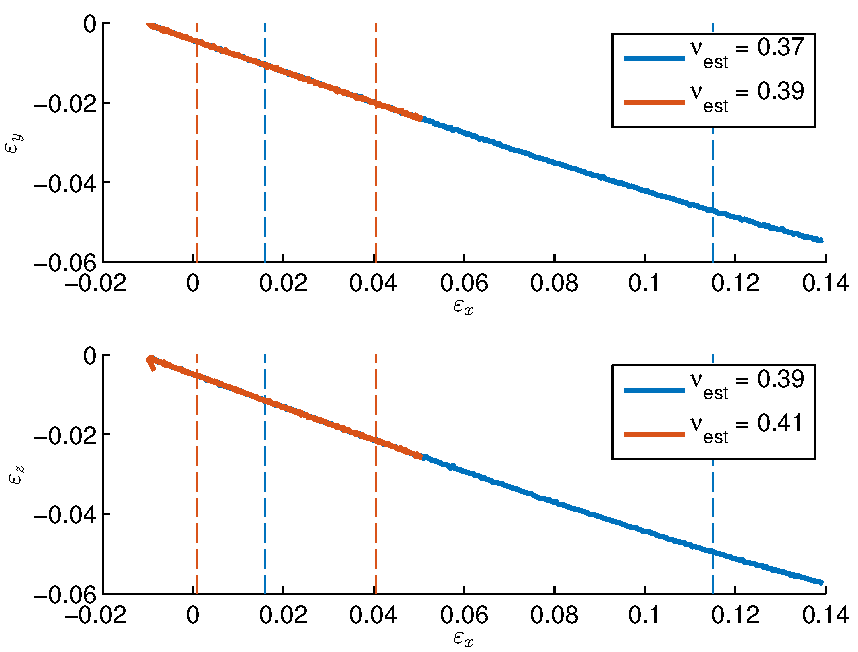
\includegraphics[width=\textwidth]{../figures/thesis/strain_strain_11_11_11_y_z_poisson_tip4p_ice_uam.pdf}
	\end{figure}
	\column{0.3\textwidth}
	Poissonforholdet er omtrent 0.4.\\
	\vspace{3mm}
	Det er litt mye. (Exp $\approx$ 0.32)
	\end{columns}
}
\end{frame}

%\subsection{}
\begin{frame}
\frametitle{Simulert system for sprekker}
\only<1>
{
	\begin{tikzpicture}[overlay, shift={($(current page.center)-(0, 0.5)$)}]
	\node (pic) at (0, 0) {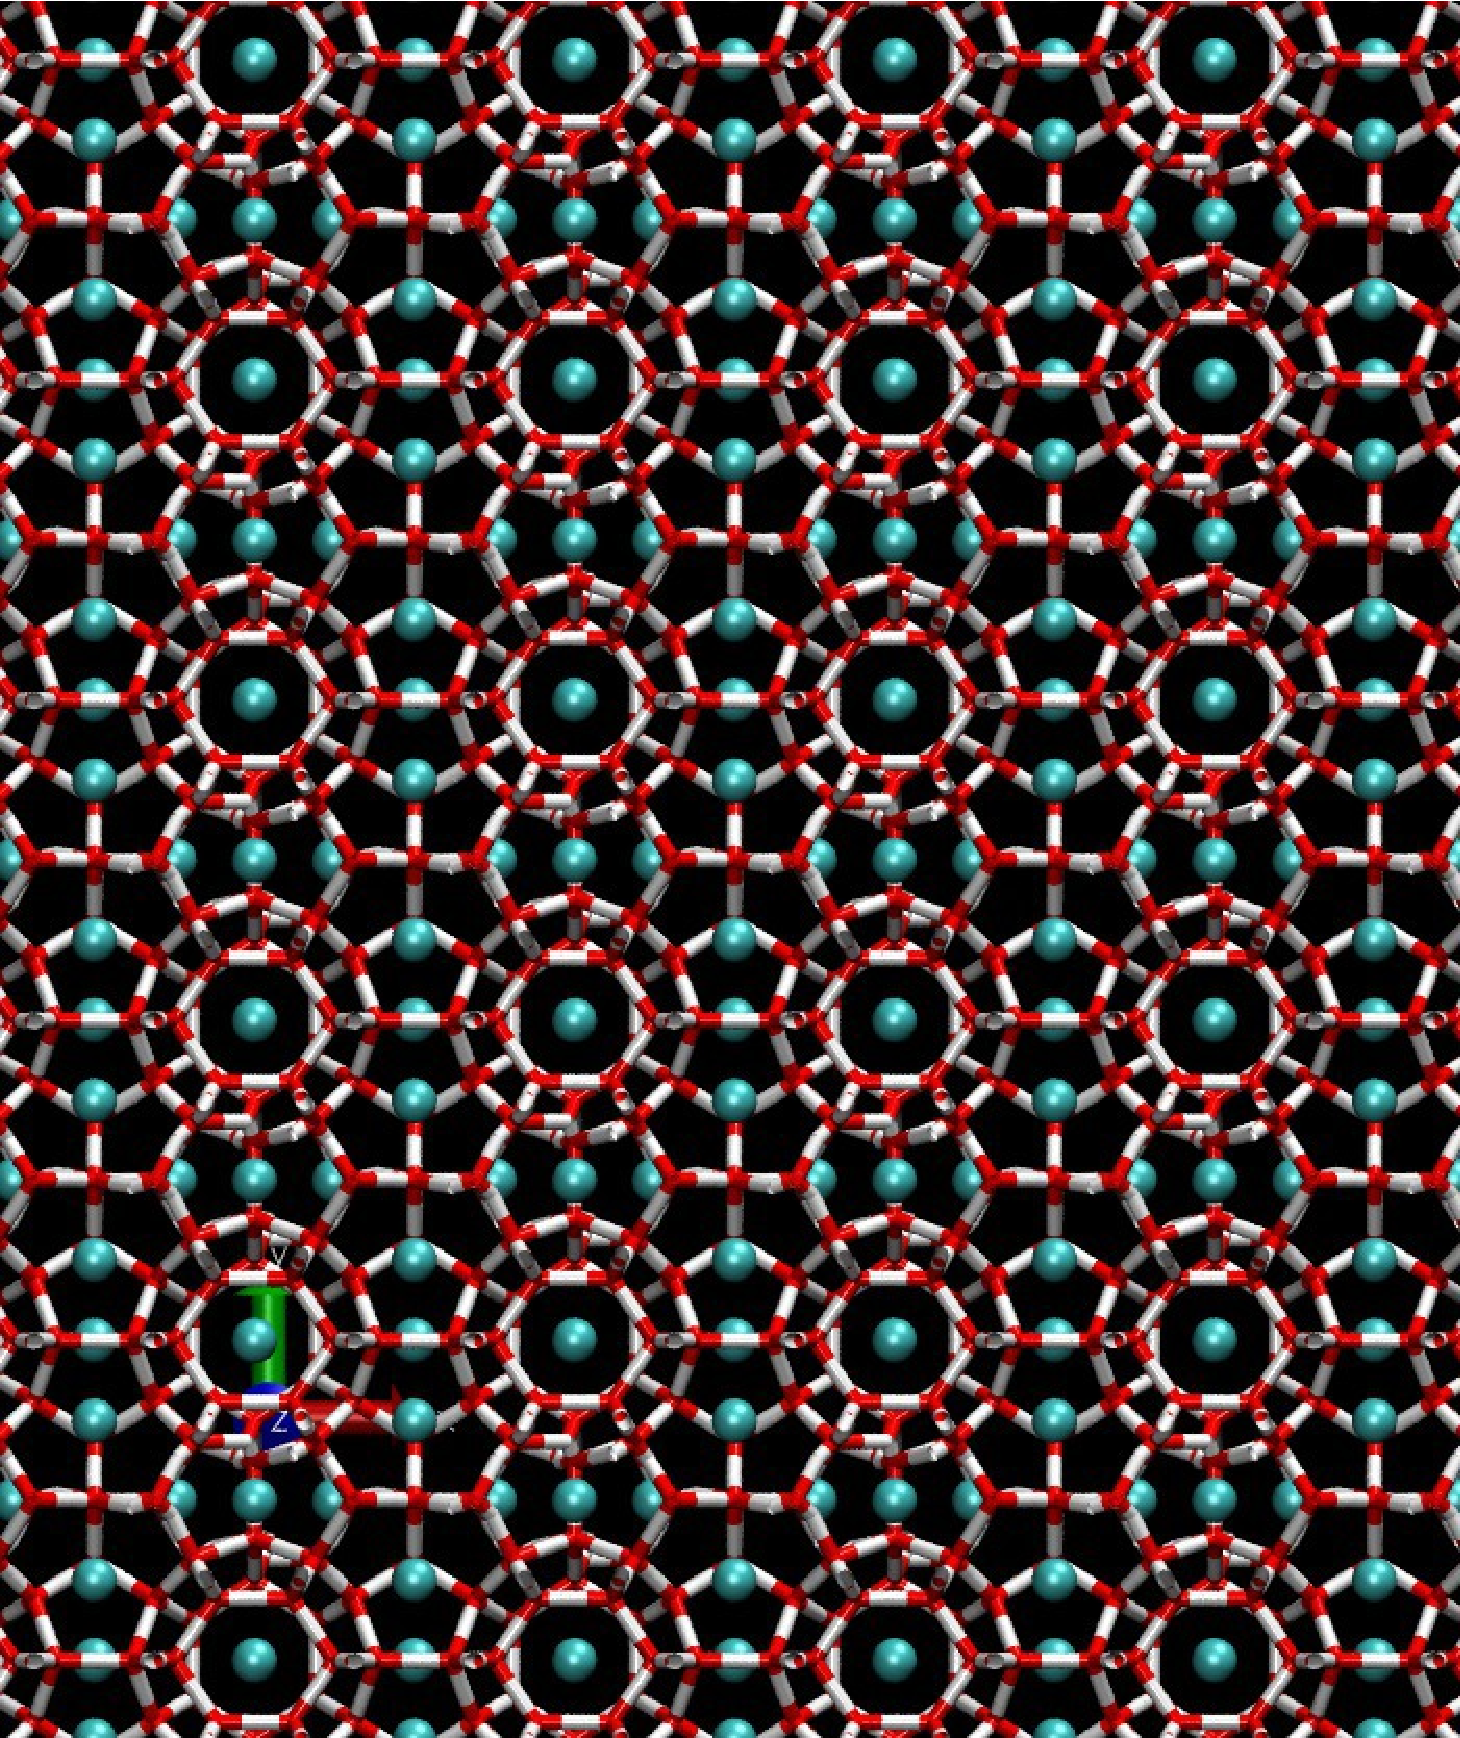
\includegraphics[trim=35 0 35 0, clip, width=4cm]{../snapshots/bulk_hydrate.pdf}};
	\end{tikzpicture}
}
\only<2>
{
\begin{tikzpicture}[overlay, shift={($(current page.center)-(0, 0.5)$)}]
\node (pic) at (0, 0) {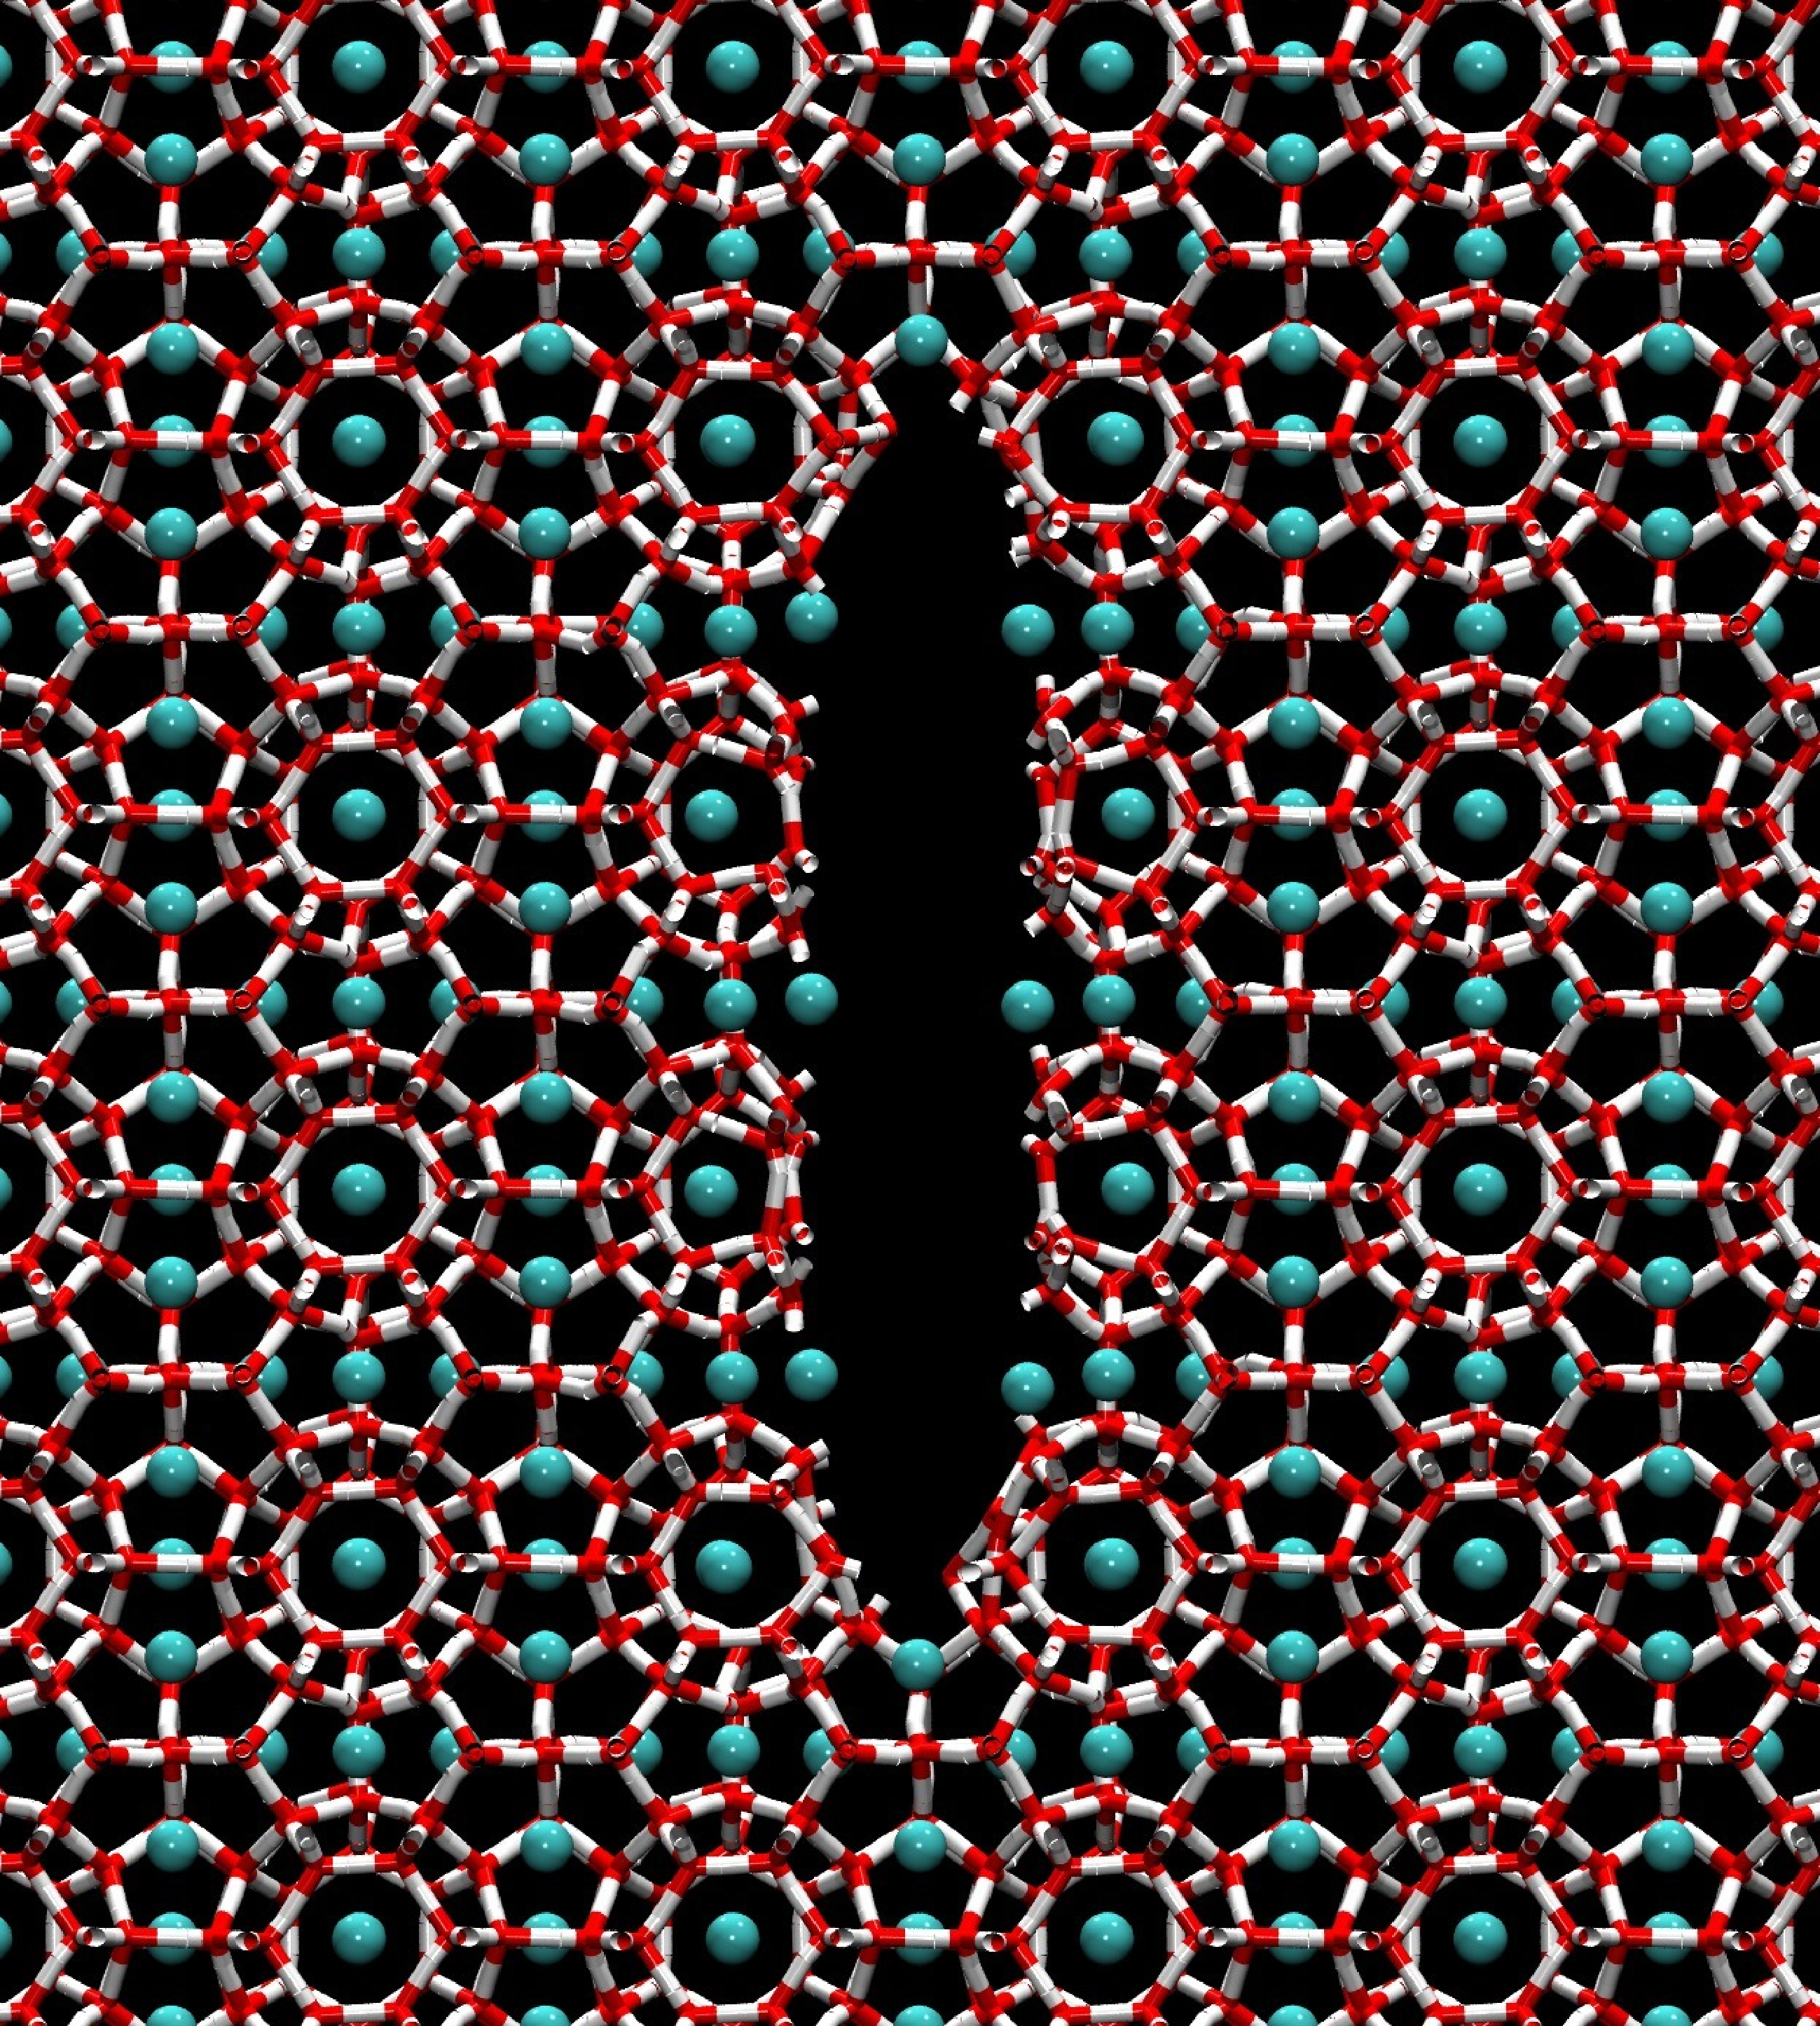
\includegraphics[trim=100 0 100 0, clip, width=4cm]{../snapshots/carved_crack.pdf}};
\end{tikzpicture}
}
\only<3>
{
\begin{tikzpicture}[overlay, shift={($(current page.center)-(2,3.5)$)}]
\centering
\filldraw[fill=blue!40!white] (0, 0) rectangle (4, 6);
\draw[very thick] (0,0) -- (4, 0);
\draw[very thick] (0,6) -- (4, 6);
\filldraw[fill=white, draw=red, thick, dashed] (2, 3) ellipse (0.25cm and 1cm);
\foreach \i in {1, 2, 3, 4, 5}
{
	\draw[thick, ->] (4, \i) -- (5, \i);
	\draw[thick, ->] (0, \i) -- (-1, \i);
}
\foreach \i in {0.3,0.6,...,3.8}
{
	\draw (\i, 0) -- (\i+0.2, -0.2);
	\draw (\i, 6.0) -- (\i-0.2, 6.2);
}
\end{tikzpicture}
}
\only<4->
{
\begin{tikzpicture}[overlay, shift={($(current page.center)-(2,3.5)$)}]
\centering
\filldraw[fill=blue!40!white] (-0.5, 0) rectangle (4.5, 6);
\draw[very thick] (-0.5,0) -- (4.5, 0);
\draw[very thick] (-0.5,6) -- (4.5, 6);
\filldraw[fill=white, draw=red, thick, dashed] (2, 3) ellipse (0.35cm and 1cm);
\foreach \i in {1, 2, 3, 4, 5}
{
	\draw[thick, ->] (4.5, \i) -- (5.5, \i);
	\draw[thick, ->] (-0.5, \i) -- (-1.5, \i);
}
\foreach \i in {-0.125, 0.25,...,4.0}
{
	\draw (\i, 0) -- (\i+0.2, -0.2);
	\draw (\i, 6.0) -- (\i-0.2, 6.2);
}
\end{tikzpicture}
}

\only<5-7>
{
\begin{tikzpicture}[overlay, shift={($(current page.center)-(2,3.5)$)},decoration={random steps,segment length=3pt,amplitude=2pt}]
\fill[white,decorate,rounded corners=1pt] (2,3) ellipse (0.15cm and 1.2cm);
\end{tikzpicture}
}
\only<6-7>
{
\begin{tikzpicture}[overlay, shift={($(current page.center)-(2,3.5)$)},decoration={random steps,segment length=3pt,amplitude=2pt}]
\filldraw[fill=white, draw=red, thick, dashed] (2, 3) ellipse (0.40cm and 1cm);
\fill[white,decorate,rounded corners=1pt] (2,3) ellipse (0.15cm and 2cm);
\end{tikzpicture}
}

\only<7>
{
\begin{tikzpicture}[overlay, shift={($(current page.center)-(2,3.5)$)},decoration={random steps,segment length=3pt,amplitude=2pt}]
\filldraw[fill=white, draw=red, thick, dashed] (2, 3) ellipse (0.45cm and 1cm);
\pgfmathsetseed{42}
\fill[white,decorate,rounded corners=1pt] (2,3) ellipse (0.20cm and 3cm);
\end{tikzpicture}
}
\only<8->
{
\begin{tikzpicture}[overlay, shift={($(current page.center)-(2,3.5)$)},decoration={random steps,segment length=3pt,amplitude=2pt}]
\pgfmathsetseed{42}
\fill[outer color=green!40!gray, inner color=white, decorate, rounded corners=1pt] (2,3) ellipse (0.23cm and 3cm) (2, 3) ellipse (0.48cm and 1cm);
\end{tikzpicture}
}
\end{frame}

\begin{frame}
\frametitle{Hva skal til for at det sprekker opp?}
\begin{block}{Griffith og Irwins energibalanse}
\begin{equation*}
\mathcal{G} > \mathcal{G}_c \stackrel{\text{sprøtt}}{=} 2\gamma_s
\end{equation*}
\end{block}
Dersom den \emph{mekaniske} energien som frigjøres ved å åpne ny sprekkflate ($\mathcal{G}$) er større enn energien som kreves for å åpne sprekken ($\mathcal{G}_c$), vil sprekken vokse.\\
\vspace{5mm}
Bruddstyrken defineres vanligvis som den mekaniske energien som må tilføres med tensilt stress for å åpne sprekkareal. Tilført energi måles ved å integrere stresset over utvidelsen:
\begin{equation} 
W = \int F \ \mathrm{d}x = A\int_{l_0}^{l_0+\Delta x} \sigma_x \ \mathrm{d}x
\end{equation}
\end{frame}

\begin{frame}
\frametitle{Bruddstyrke}
\begin{equation*}
\mathcal{G}_c \approx 0.4 \text{ J/m}^2
\end{equation*}
\begin{equation*}
K_{Ic} \approx 0.06 \text{ MPam}^\frac{1}{2}
\end{equation*}
\vspace{5mm}
\center{Dette betyr at en sprekk vil løpe dersom det å åpne en kvadratmeter med sprekk fører til at det frigjøres 0.4 Joule med \emph{mekanisk} energi.}
\vspace{5mm}
\center{Resultatet er omtrent det samme som eksperimentelle resultater for vanlig is.}
\end{frame}


\begin{frame}
\frametitle{Hva var det vi lurte på?}
\begin{itemize}
\item Bruddstyrke -- funnet
\item Sprøtt eller duktilt? -- Sprøtt
\item Bruddmekanisme -- Kommer
\item Frigjort metan -- Kommer
\end{itemize}
\end{frame}


%\subsection{}
\begin{frame}{Måling av arealet til sprekkoverflaten}
\begin{columns}[c]
\column{0.5\textwidth}
Jeg bruker en Monte-Carlo-metode for å finne tilgjengelig overflate:
\begin{equation*}
A_{s} = 2V\frac{n_s}{L}
\end{equation*}
\begin{table}
\begin{tabular}{ll}
$A_{s}$ & overflatearealet \\
$V$ & volum av prøven \\
$n_s$ & antall krysninger vegg--tomrom \\
$L$ & total lengde av trukne linjestykker 
\end{tabular}
\end{table}

\column{0.5\textwidth}
	\begin{figure}
 	\centering
 	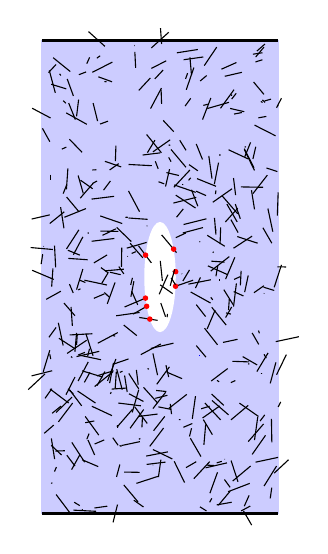
\begin{tikzpicture}
 		\filldraw[blue!20!white] (0, 0) rectangle (3, 6);
 		\draw[very thick] (0,0) -- (3, 0);
 		\draw[very thick] (0,6) -- (3, 6);
 		\fill[name path=myellipse, white] (1.5, 3) ellipse (0.2cm and 0.7cm);
 		\pgfmathsetseed{1138}
 		\foreach \x in {1,2,...,400} 
 		{
 			\pgfmathrandominteger{\a}{0}{300}
 			\pgfmathrandominteger{\b}{0}{600}
 			\pgfmathrandominteger{\c}{0}{359}
 			\pgfmathrandominteger{\d}{0}{180}
 			\pgfmathsetmacro{\length}{0.3*cos(\d)}
% 			%\def\length{\pgfmathresult}
 			\draw[name path=myline] (\a/100,\b/100) -- ++(\c:\length);
 			\def\n{0}
 			\fill [execute at begin node={\global\let\n=\n}, name intersections={of = myline and myellipse, total=\n}];
 			\pgfmathifthenelse{\n==1}{"\noexpand\fill [red] (intersection-1) circle (1pt)"}{"\noexpand\fill [blue] (2, 2) circle (0pt)"}
 			\pgfmathresult;
 		}
 	\end{tikzpicture}
	\end{figure}
	\end{columns}
	\myref{Likning: Forenklet fra Bhattacharya et. al, Langmuir, 25(10), 2009}
\end{frame}

%\subsection{}
\begin{frame}
\frametitle{Bruddmekanisme}
\begin{figure}
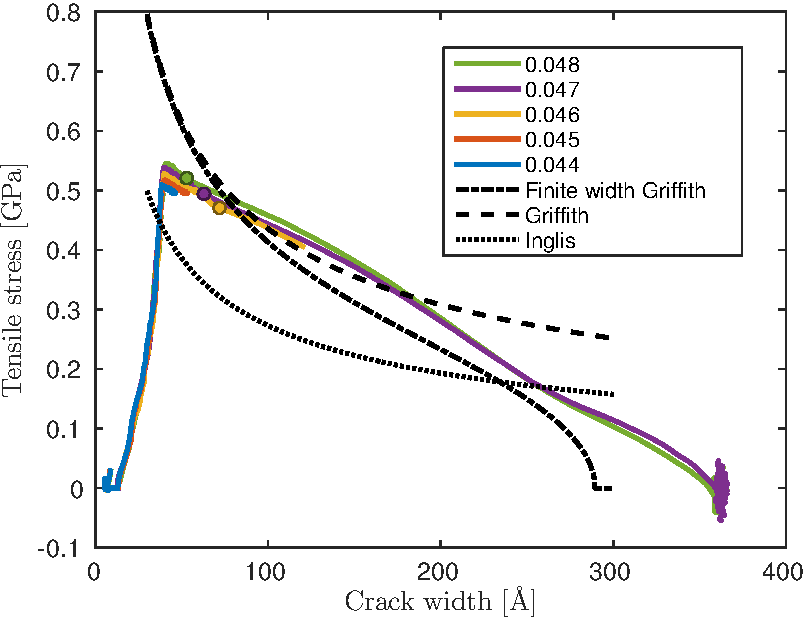
\includegraphics[width=0.9\textwidth]{../figures/thesis/fracture_theory_compare.pdf}
\end{figure}

\end{frame}

\begin{frame}
\frametitle{Frigjøring av metan: metan frigjøres fort under oppsprekking}
\begin{figure}
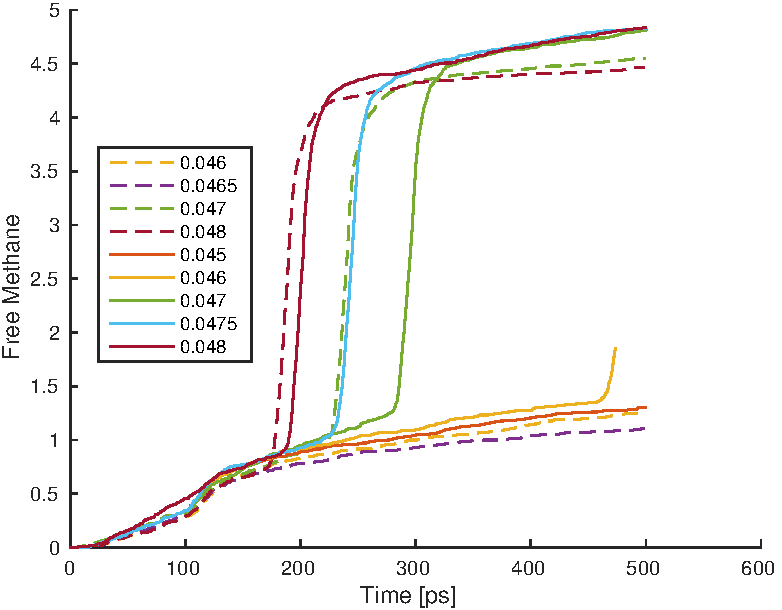
\includegraphics[width=0.9\textwidth]{../figures/thesis/released_methane_temp.pdf}
\end{figure}
\end{frame}



\section{Oppsummering}
\subsection{}
\begin{frame}
\frametitle{Oppsummering}
\begin{itemize}
\item Jeg har gjort sprekksimuleringer av gasshydrater med molekylærdynamikk
\item Bruddstyrken er omtrent 0.4 J/m$^2$
\item Gasshydratene mine er sprø, men smelting er en viktig del av sprekkprosessen.
\item Metan frigjøres fort, men vi vet fortsatt lite om hvilken rolle det frigjorte metanet har.
\end{itemize}
\end{frame}

\end{document}